% Kapitel 9 - Fazit
\section{Implementation}
In chapter \ref{sec:Algorithm definition}, a comprehensive and exhaustive study of different approaches to compression algorithm was conducted. The conclusion drawn was that an approach with mathematical reduction with a combination of data filtering was the most suitable for the type of data-sets being dealt with in this thesis, i.e .asc files. In this chapter, the implementation of the conclusion from previous chapter would be discussed.

\subsection{Algorithm Selection}
As per previous chapter, real time processing via mathematical reduction is the most suitable method to achieve optimal fulfillment of the requirements. The implementation of this method requires to easy access to :
%\ref{fig:Weighted Analysis}
\begin{itemize}
    \item Test systems with CANoe pre-installed
    \item CAPL coding environment
    \item Data files for testing and validation
\end{itemize}

CANoe is a licensed tool provided by Vector Informatik GmbH. It is a complex and large tool to use with numerous features suitable for different types of uses in diversified environments in the domain of verification \& validation. The licenses are extremely expensive and hence the easy access to such tools is also restricted. Usually such licenses are purchased in limited quantities and shared in team pools for various projects and hence the access is always determined by priority of implementation basis. 

Vector provides three types of licensing for CANoe tool, each of which have their own utilities and limitations. The three types of licenses are :

\begin{itemize}
    \item CANoe pro
    \item CANoe run
    \item CANoe pex
\end{itemize}

The pro version is the highest tier license version of CANoe. As the name suggests, the license gives access to all features of CANoe tool which also includes CAPL coding environment. The run license provides limited access to CANoe environment where it is possible to run and analyse all the pre-existing test setups and programs. The user is restricted from changing any configurations in the setups using run license. The pex license is the basic license required to view CANoe tool. It is useful for viewing the tool and it's setup and configurations, however, creating, running or changing configurations and setups are prohibited. Here, \ref{fig:CANoe Licenses}, one can see the features included with pro license.

\begin{figure}[h]
    	\centering
    	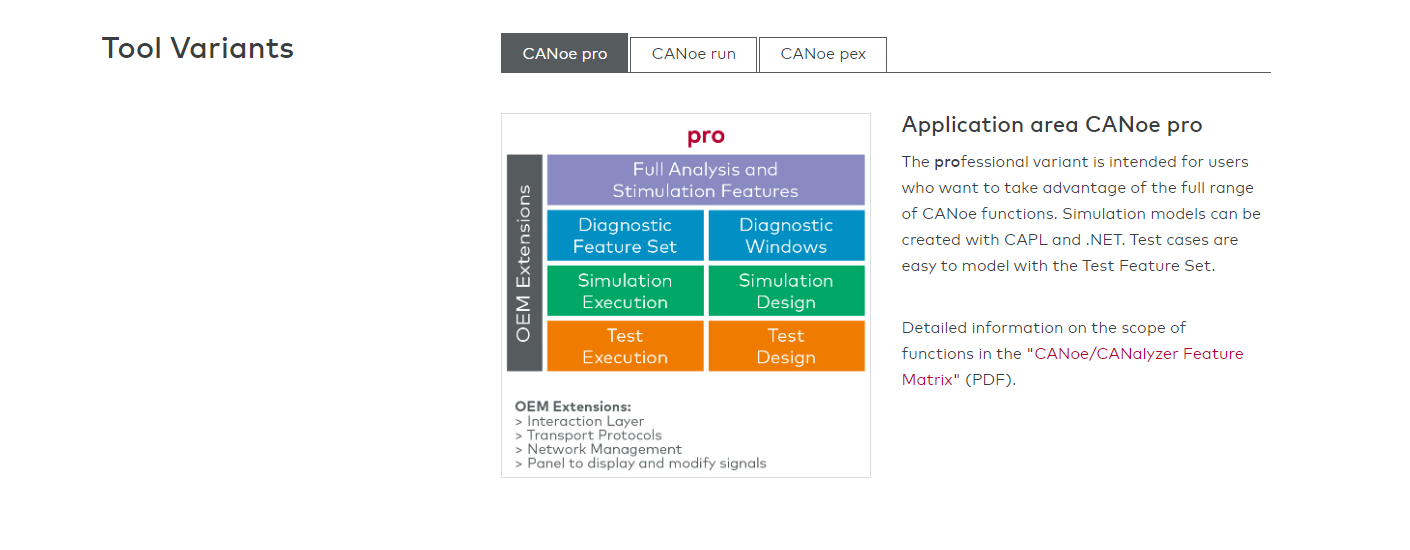
\includegraphics[width= 1\textwidth]{images/CANoe license type.png}
    	\caption [Licenses]{CANoe licenses}  
    	\label{fig:CANoe Licenses}
\end{figure}

\begin{figure}[h]
    	\centering
    	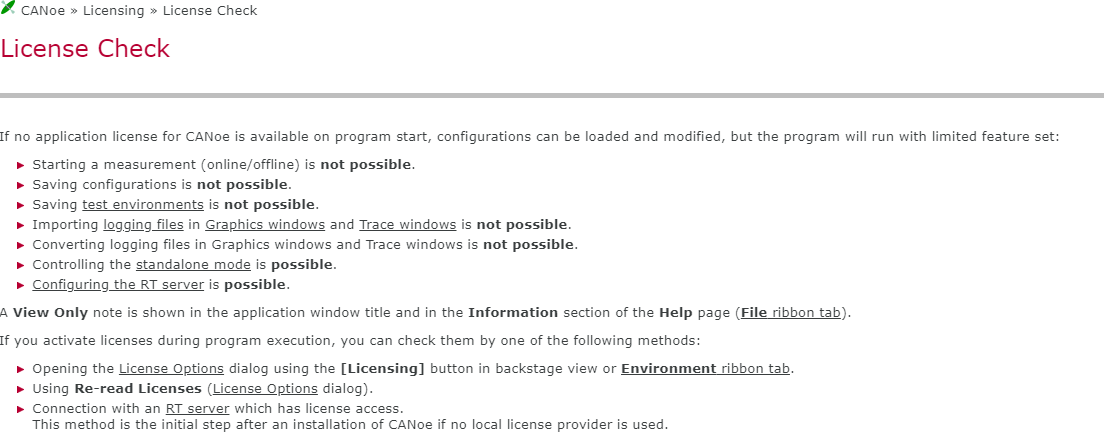
\includegraphics[width= 1\textwidth]{images/CANoe license restrictions.png}
    	\caption [Restrictions]{CANoe restrictions}  
    	\label{fig:CANoe Restrictions}
\end{figure}


\clearpage

Figure \ref{fig:CANoe Restrictions} shows the restrictions involved with limited access licenses. Hence, it is of utmost importance to have access to the pro version of licenses. At CES, CANoe pro licenses are available to use for test systems. However, it is subjected to availability of the test systems. Since, multiple projects require the availability of test systems, getting a free-to-use access to test systems is difficult. Since, implementing the algorithm requires constant access to development environment for development, testing and validation an alternative was required to overcome the limited access to the test systems. 

As discussed in the conclusion of \ref{sec:Algorithm definition}, the weighted analysis revealed two possible alternatives for implementation of mathematical reduction based compression algorithm : \\
1) Real Time Processing    2) Batch Processing or Post-Processing 

Since, the approach for compressing data and reducing data size in both processes is identical, the use of an alternative to the real time processing approach can be considered and tested to verify if the desired compression is achieved or not. Once, the data compression is verified and validated, the algorithm can be transferred from post-processing to real-time processing with necessary changes. This will be discussed as part of scope of development for future.

To conclude, the compression algorithm with post processing will be used as the base for implementation study and the development platform to be used for this purpose will be python.

But before moving to development phase, it is necessary to define the structure of the program. Without a proper structure, it is easy to lose the sight of goal or worse get entangled in unproductive development hassles irrelevant to the goals. Designing the structure of a program before starting to code is an important step in the software development process. It can help ensure that the code is well-organized, maintainable, and easy to understand. Here are some common ways to design the structure of a program: 

\begin{itemize}
    \item Pseudo-code: Pseudo-code is a high-level, human-readable description of the steps a program should take to solve a problem. It is written in a syntax that resembles a programming language but is not meant to be executed. Pseudo-code can be a useful tool for designing the structure of a program, as it allows you to think through the problem and get a rough idea of the steps your code will need to take before writing any actual code.
    \item Flowcharts: A flowchart is a picture of the separate steps of a process in sequential order. It is a generic tool that can be adapted for a wide variety of purposes, and can be used to describe various processes, such as a manufacturing process, an administrative or service process, or a project plan \cite{Flow}
    \item Mind maps: Mind maps are diagrams that show the relationships between different ideas or concepts. They can be used to design the structure of a program by breaking the problem down into smaller parts and showing how they fit together. Mind maps can be a good way to get a bird's eye view of the program and see how all of the pieces fit together.
    \item Diagrams and schematics: You can also use other types of diagrams and schematics to design the structure of a program. For example, you might use a block diagram to show the relationships between different parts of the program, or a state diagram to show the different states that a program can be in and the transitions between those states.
    \item Code sketching: Finally, you can also start designing the structure of a program by sketching out some of the code on paper. This can be a good way to experiment with different approaches and see what code structures make the most sense for the problem you are trying to solve.
\end{itemize}

For the purpose of algorithm design and road-map, a flowchart was selected and the same will be discussed below. Flowcharts are pictorial representation of the flow of design/development process. Flowcharts can be used to explain system-level development as well as detailed in depth process of design depending on the requirements. Symbols are key aspects of a flowchart as each symbol represents certain process or logic in the program. Below are some of the most commonly used symbols in a flowchart design : 


\begin{figure}[!h]
    	\centering
    	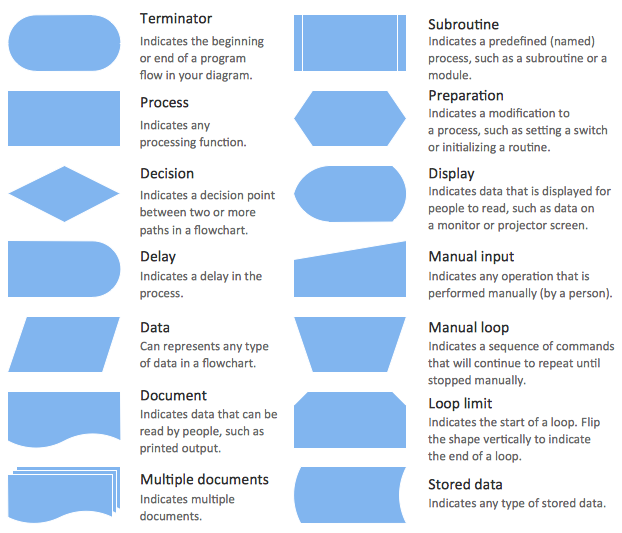
\includegraphics[width= 0.9\textwidth]{images/Design-Elements-Flowchart1.png}
    	\caption [Flowchart Symbols - I]{Flowchart Symbols - I}  
    	\label{fig:Flowchart Symbols}
\end{figure}

\clearpage

\begin{figure}[h]
    	\centering
    	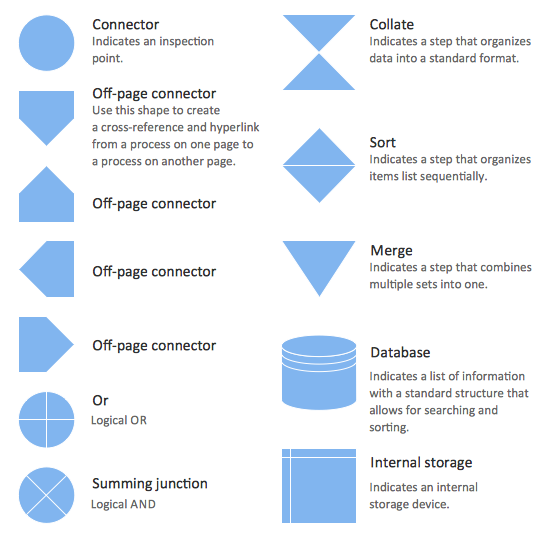
\includegraphics[width= 0.9\textwidth]{images/Design-Elements-Flowchart2.png}
    	\caption [Flowchart Symbols - II]{Flowchart Symbols - II}  
    	\label{fig:Flowchart Symbols}
\end{figure}

The flowchart used for design process is intended to show the three parts of the algorithm design : 

\begin{itemize}
    \item Primary Code
    \item Arithmetic Reduction Unit
    \item Data Evaluation Tools
\end{itemize}

\newpage
The below figure shows the flow of the primary code. The primary module of the program is designed to work as an interface between the user, system and data-sets. As seen in the figure, the program will seek user input at execution. The user input will be the key aspect in setting various parameters such as tolerance windows, program run time etc. Once the user has input values to the program, it will enter monitoring phase. The program will monitor every single file added into the destination folder and then when it finds eligible file types, it will read, process and parse the data from these files. The parsed data is then passed into 3 sub modules , two for mathematical reduction and one for data evaluation. Once the parsed data is processed and compressed by these sub modules, it is output for user evaluation via an excel file thus culminating the data compression method.

\begin{figure}[H]
    \centering
    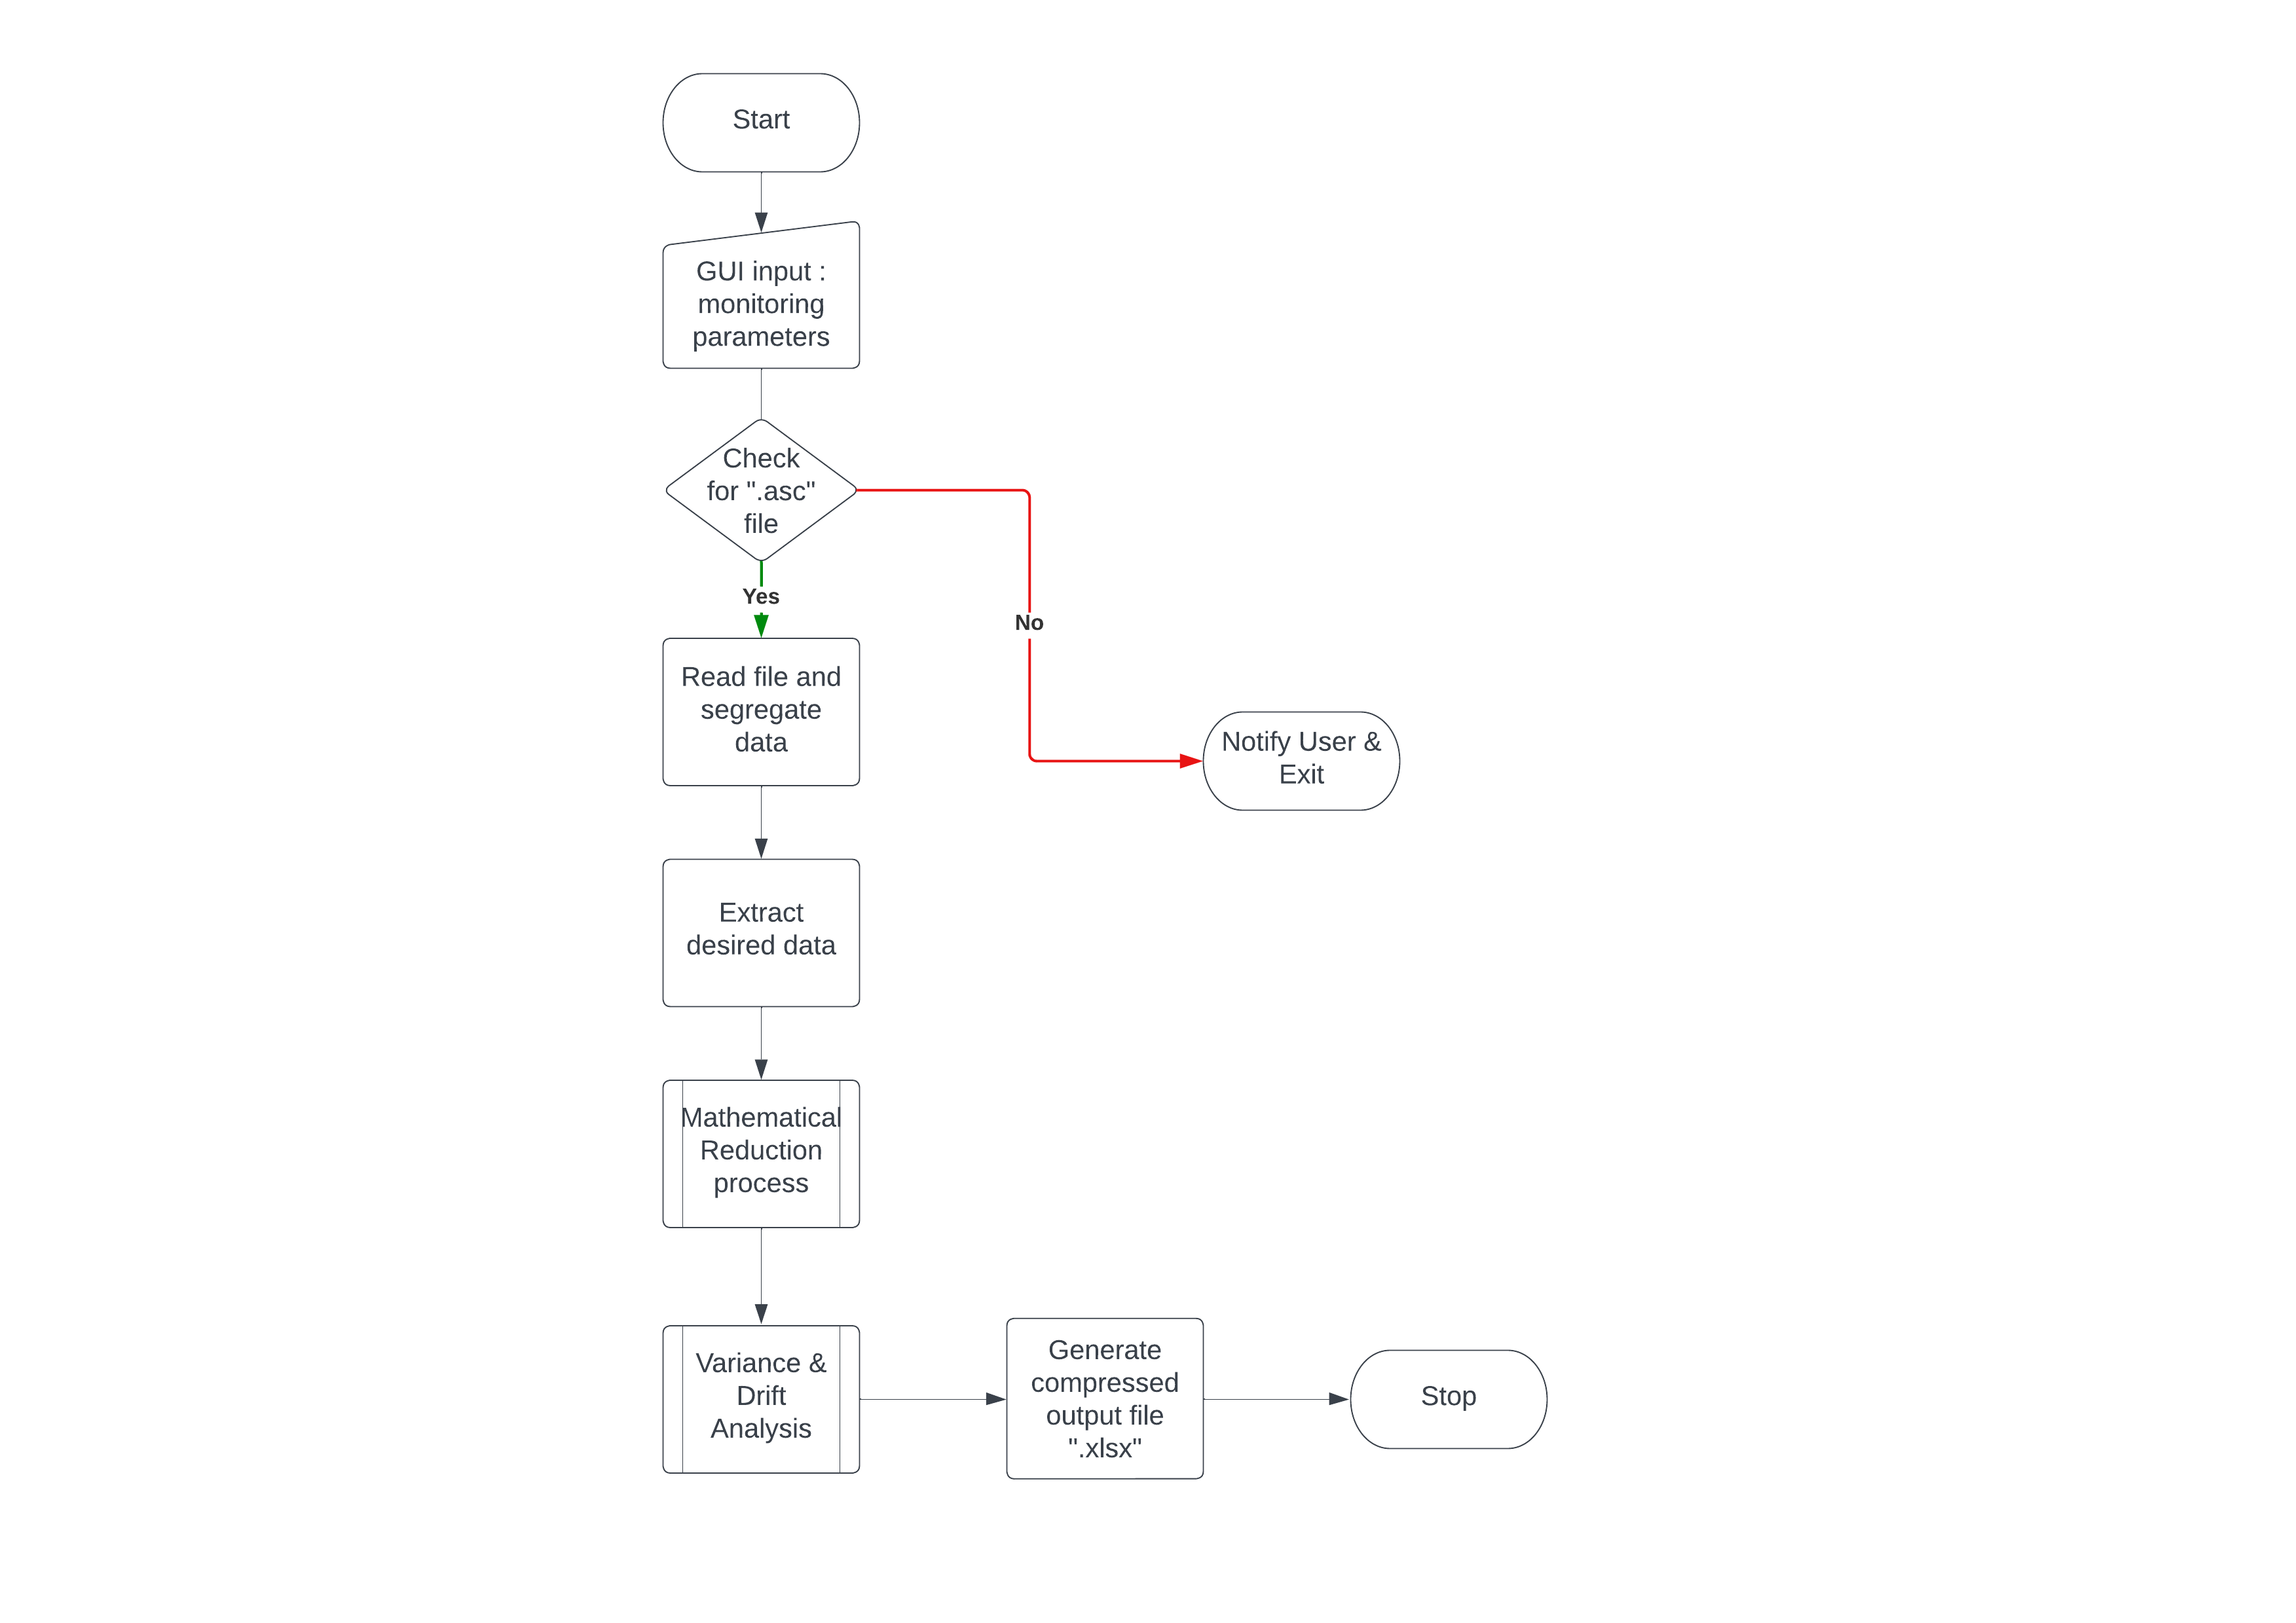
\includegraphics[width= 0.8\textwidth]{images/Overview-algo.png}
    \caption [Algorithm Overview]{Algorithm Overview}  
    \label{fig:Algo-I}
\end{figure}

The Mathematical reduction algorithm shown below has a very straightforward approach in the sense, it gets invoked by the main module, processes data passed on by the function call, and returns the output in form of reduced data. The sub routine indicated by "A" shows the detailed description of mathematical reduction process. The primary conditional check is determined by operation mode. Based on operation mode, corresponding parametric value and tolerance values are set. Once the values are set, the filtering begins followed by arithmetic mean process and at the end a reduced data-set is obtained. 

\begin{figure}[H]
    \centering
    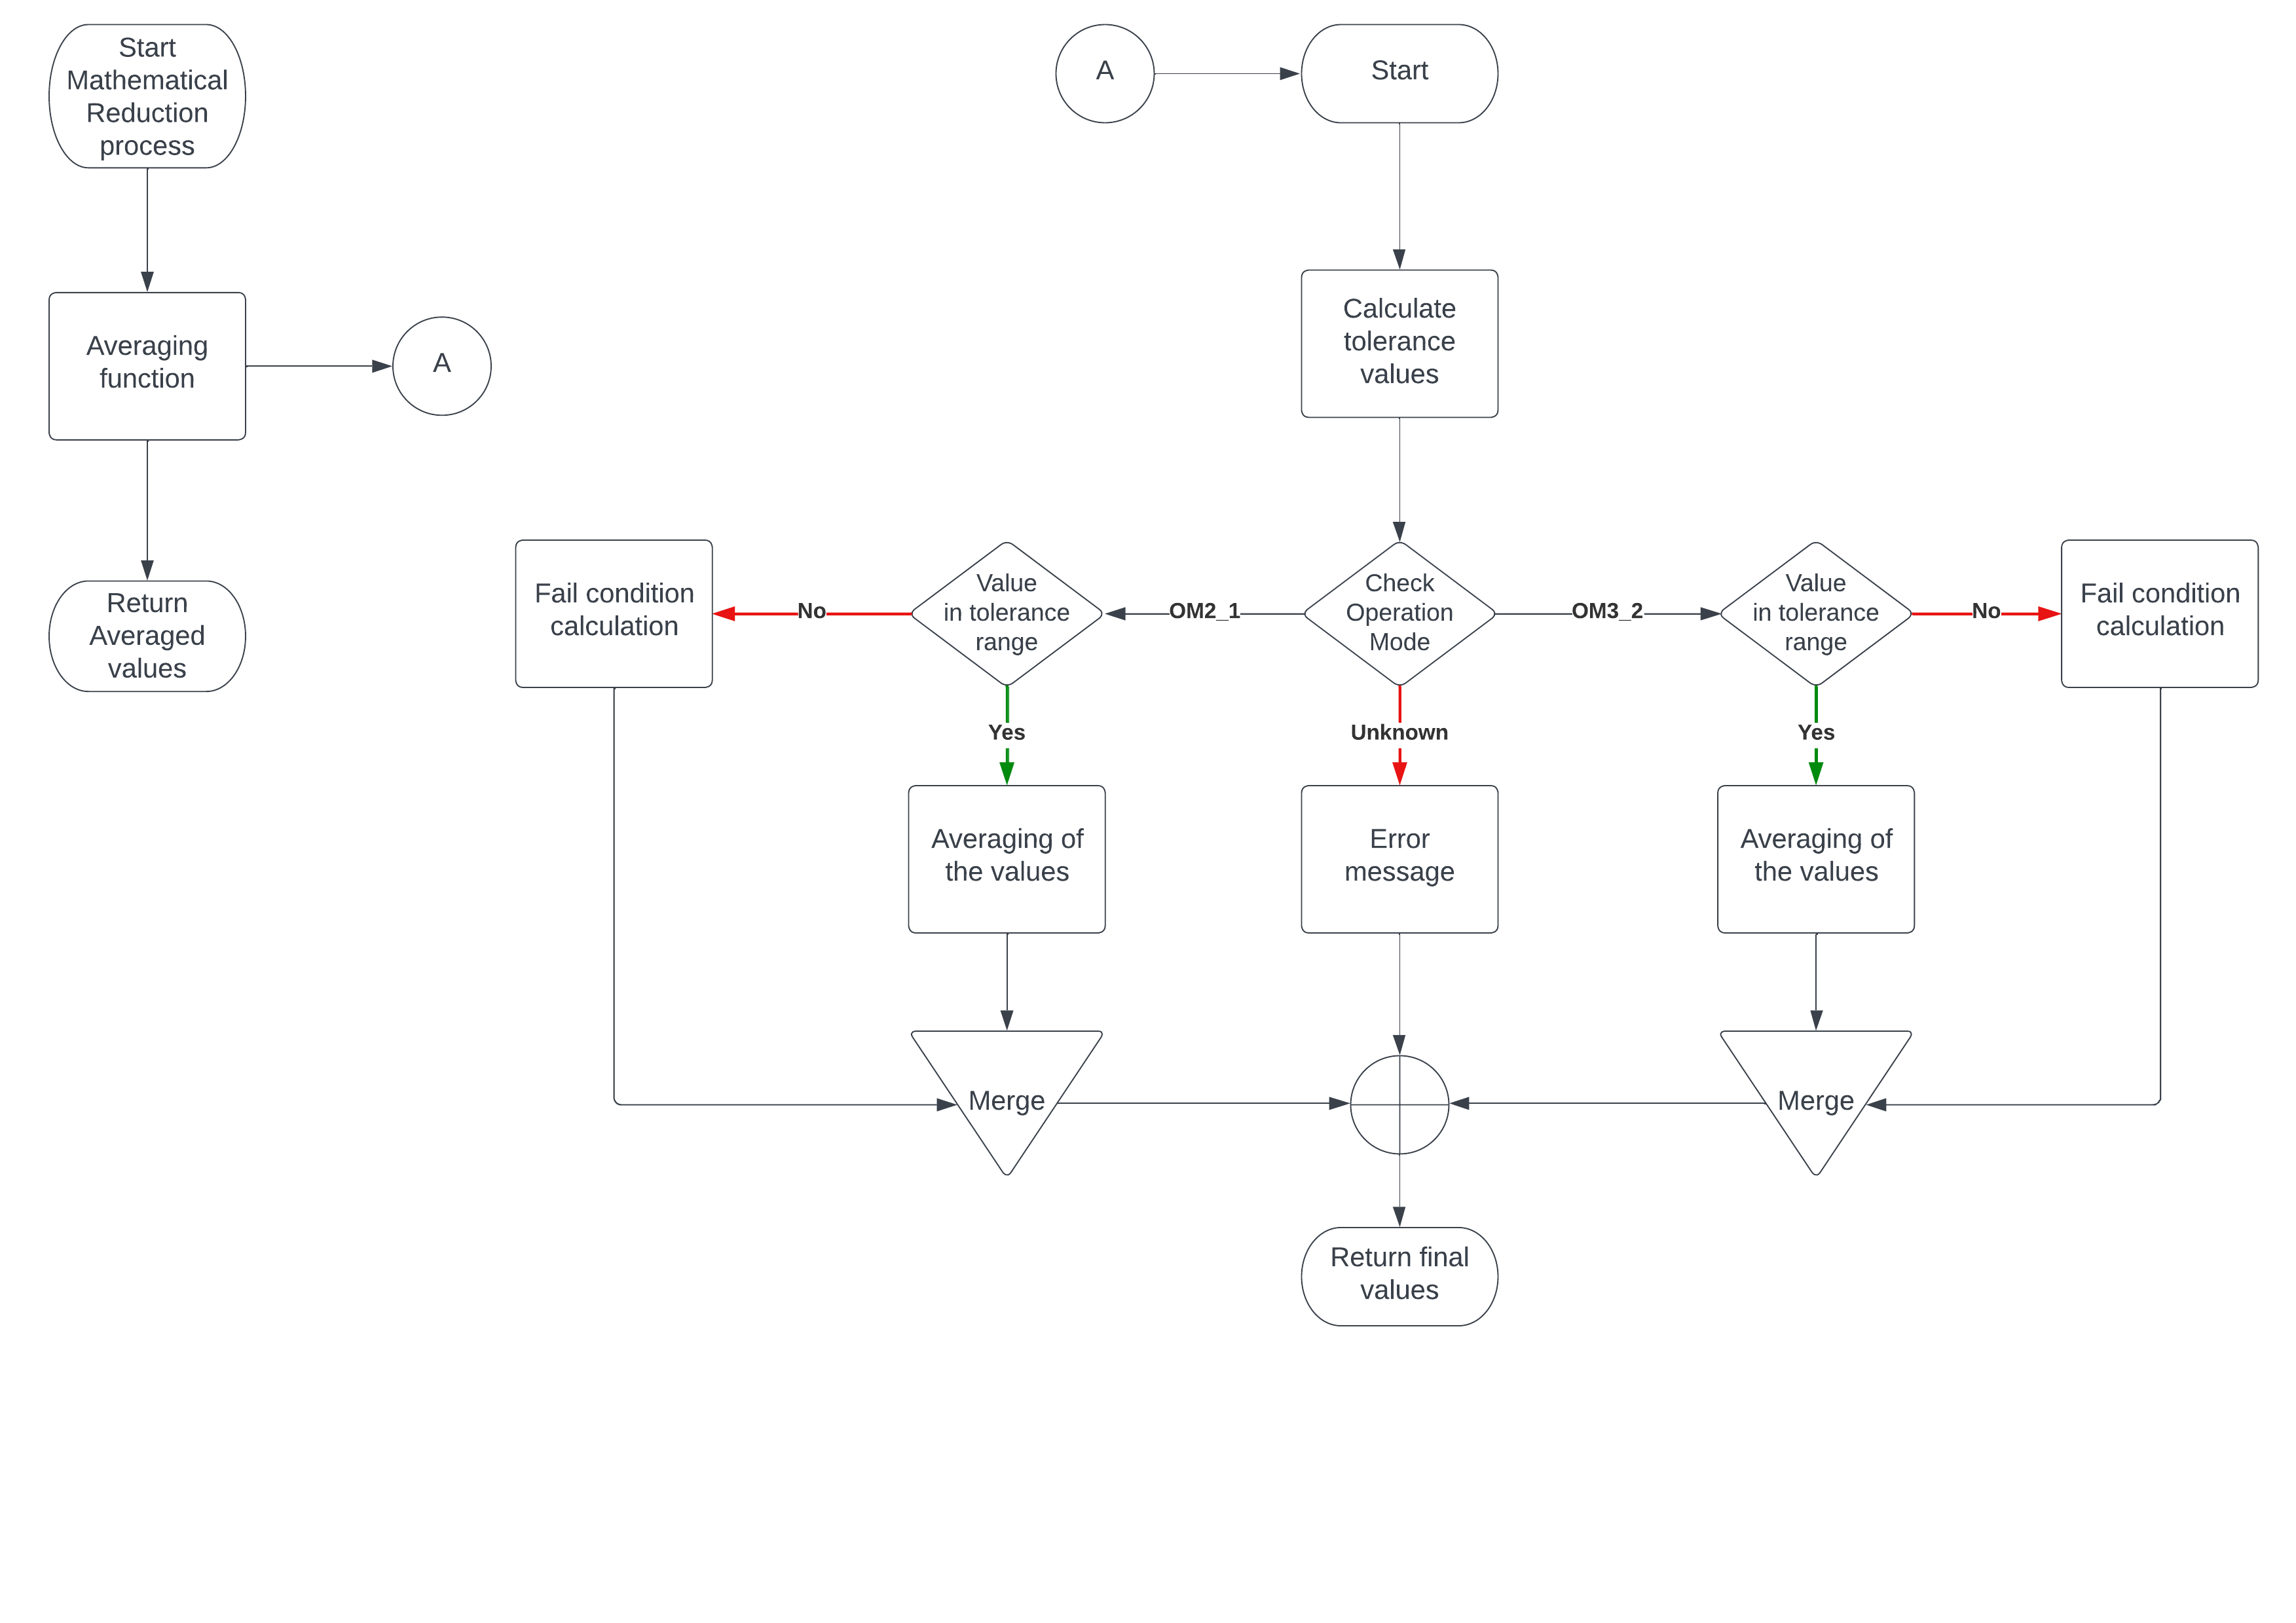
\includegraphics[width= 0.9\textwidth]{images/MathematicalProcess.png}
    \caption [Mathematical Reduction]{Mathematical Reduction Flowchart}  
    \label{fig:Mathematical Reduction}
\end{figure}


The following algorithm indicates two data evaluation methods implemented via this program. The first one calculates the variance of the reduced error free data-set. The second method is the drift analysis method. The error free reduced data-sets are split into smaller groups or samples and then quantise them by calculating mean of these samples. The drift analysis functions returns these quantised samples to the function call.

\begin{figure}[H]
    \centering
    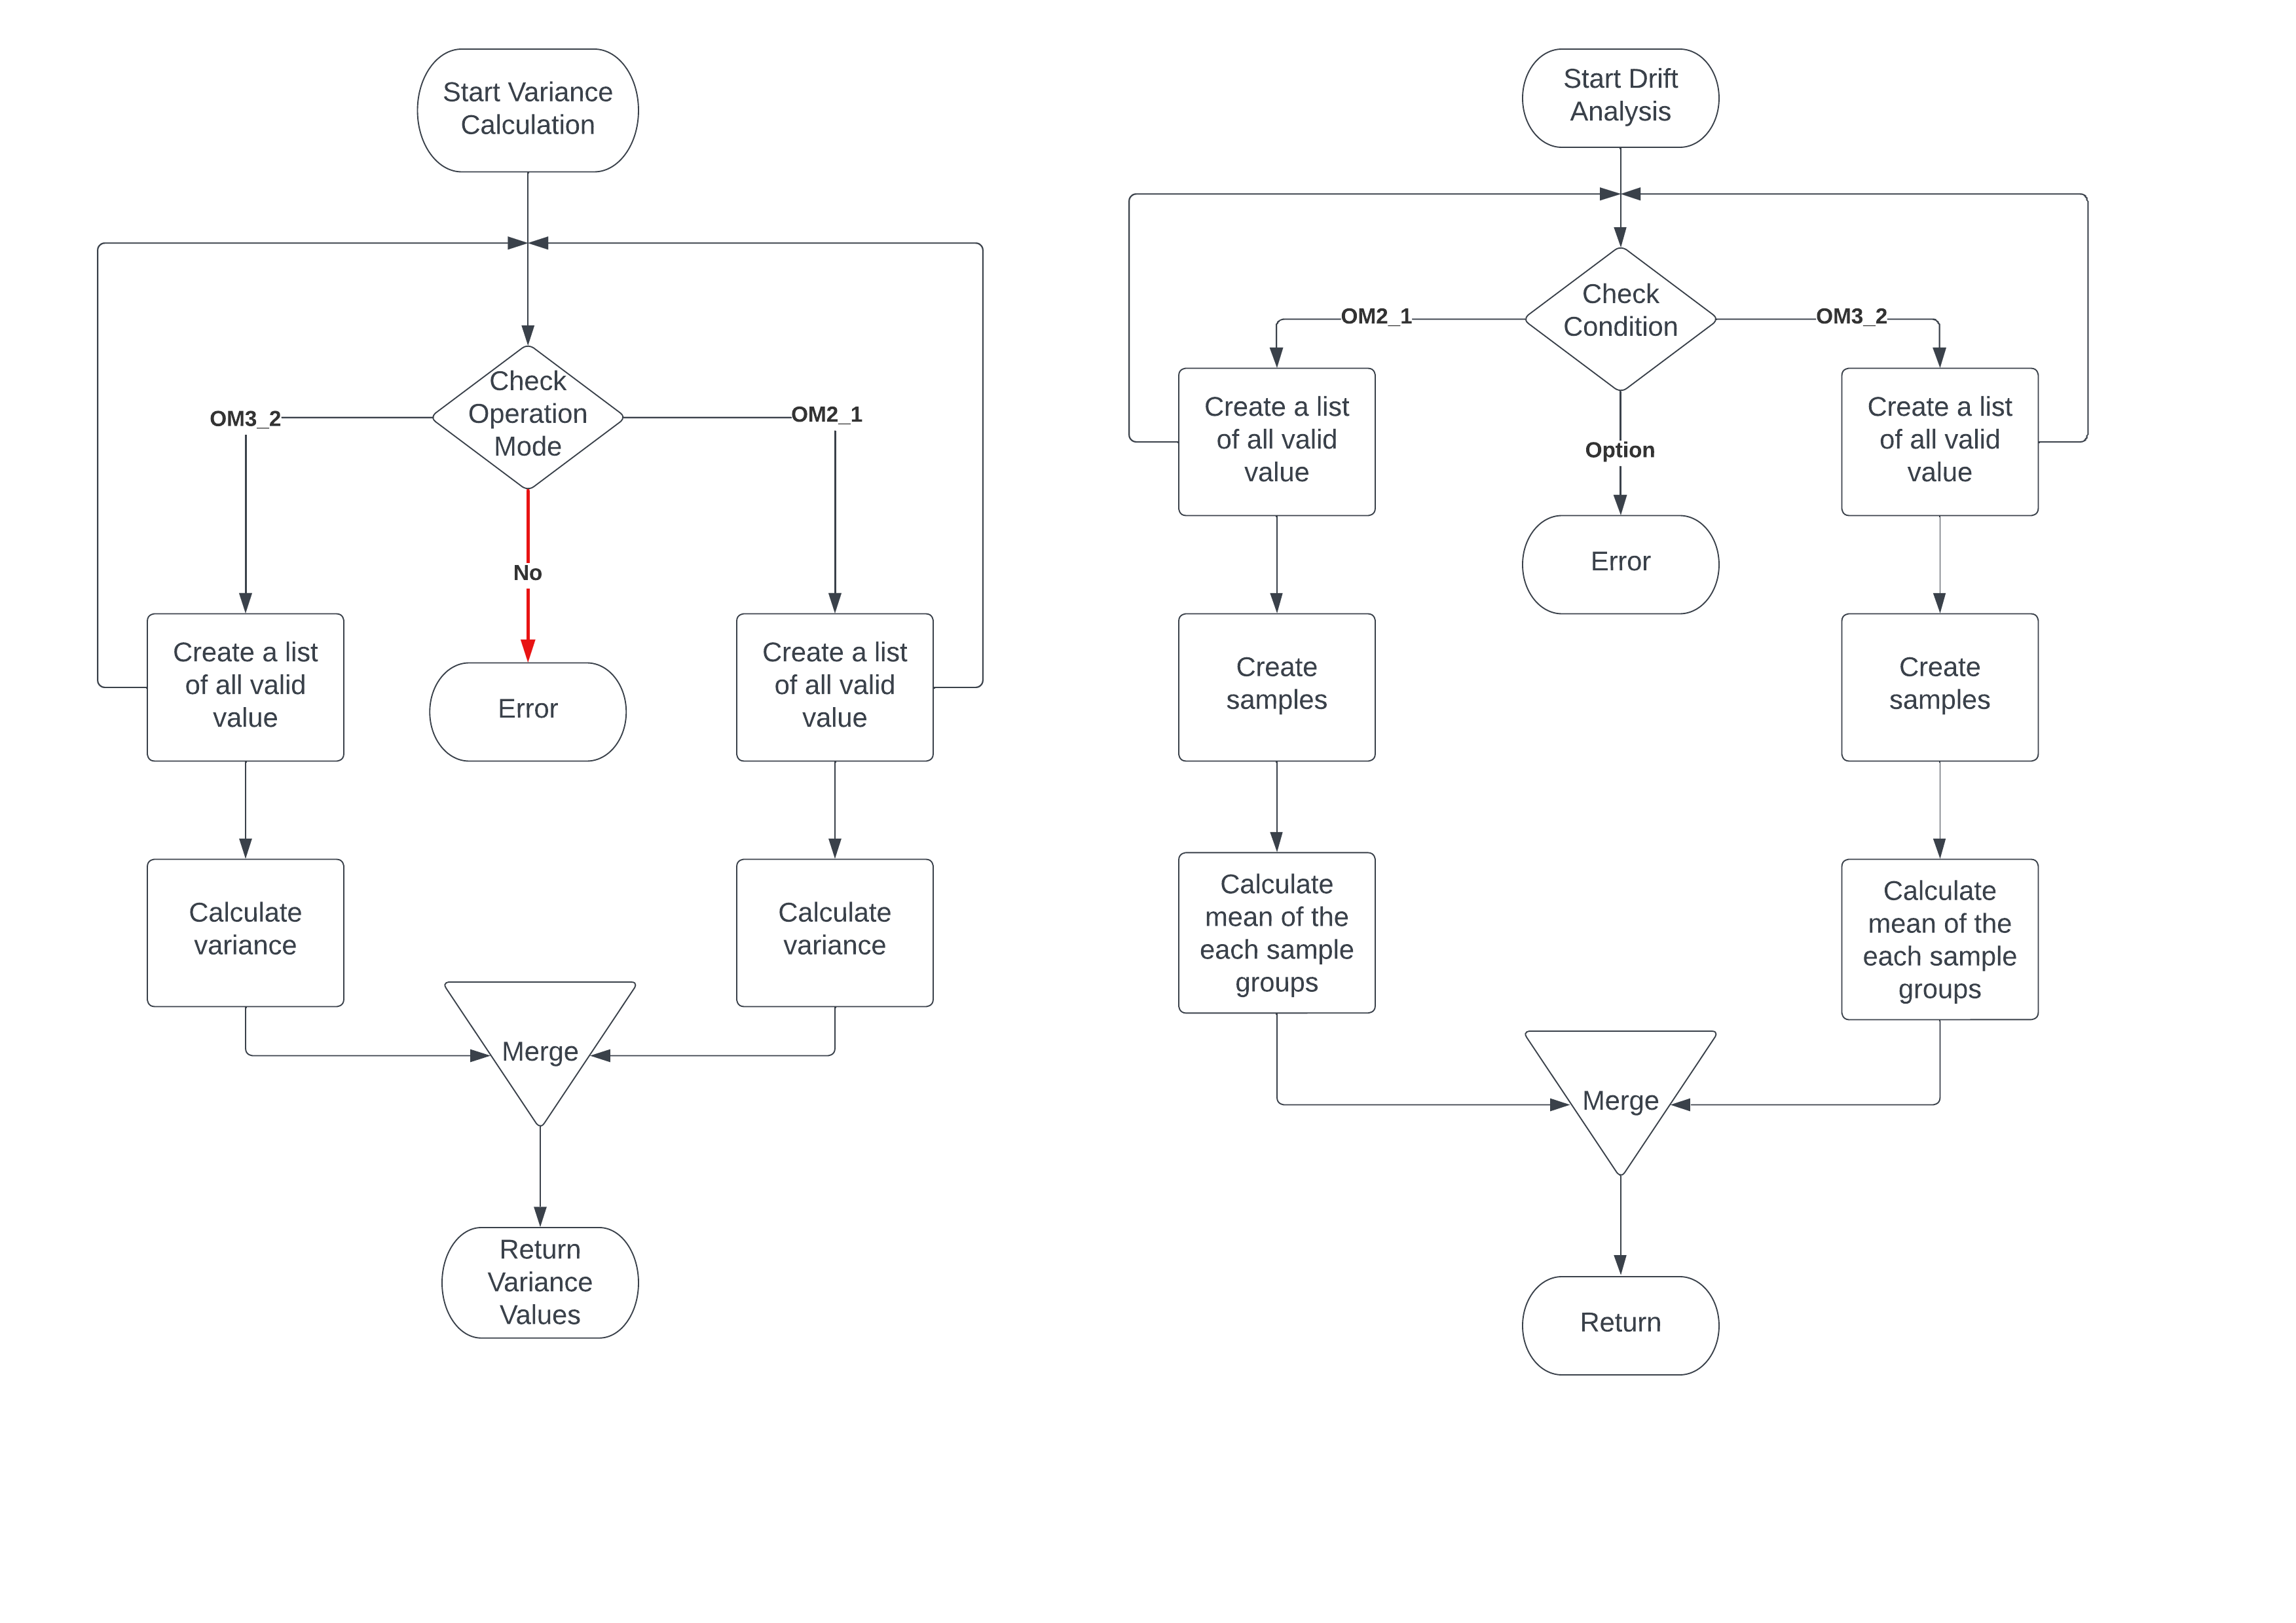
\includegraphics[width= 0.9\textwidth]{images/Drift.png}
    \caption [Drift Analysis]{Variance \& Drift Analysis}  
    \label{fig:Drift Analysis}
\end{figure}

Now that the final selection of algorithm, work environment and program design is accomplished, the next step is to introduce the initial setup before implementing the algorithm. 
\newpage

\subsection{Initial Setup}

Python is a high-level, interpreted, general-purpose programming language. It was first released in 1991 by Guido van Rossum and has since become one of the most widely used programming languages in the world.

Python is popular for its simple, easy-to-read syntax which allows developers to express concepts in fewer lines of code compared to other programming languages. It is also highly versatile and can be used for a variety of applications, including web development, scientific computing, data analysis, artificial intelligence, and more. One of the main benefits of using Python is its extensive library of modules and packages, which makes it easy to perform common programming tasks without having to write extensive amounts of code. This has led to a large and active community of developers who continuously contribute to the development and improvement of the language.

There are currently two stable versions of Python in widespread use: Python 2 and Python 3. Python 2 was first released in 2000, and although it is still in use, its development has been largely discontinued in favor of Python 3. Python 3 was first released in 2008 and has since become the standard version of Python, with many improvements over Python 2. The compression algorithm discussed in this thesis has thus been designed exclusively using Python 3. 

Python programs can be written and executed by means of a terminal or IDE also known as Integrated development environment. The scripts, or codes, are written and saved with a ".py" extension. An IDE was selected and utilized for the purpose of development of compression algorithm in this thesis. An integrated development environment (IDE) is a software application that provides comprehensive facilities to computer programmers for software development. An IDE normally consists of at least a source code editor, build automation tools and a debugger \cite{PyWiki}. IDEs maximize user productivity by providing easy access to multiple components of the coding environment such as code alignment, errors \& warnings indicators, easy install of packages library etc.   

One aim of the IDE is to reduce the configuration necessary to piece together multiple development utilities. Instead, it provides the same set of capabilities as one cohesive unit. Reducing setup time can increase developer productivity, especially in cases where learning to use the IDE is faster than manually integrating and learning all of the individual tools. Tighter integration of all development tasks has the potential to improve overall productivity beyond just helping with setup tasks. For example, code can be continuously parsed while it is being edited, providing instant feedback when syntax errors are introduced, thus allowing developers to debug code much faster and more easily with an IDE.

Some IDEs are dedicated to a specific programming language, allowing a feature set that most closely matches the programming paradigms of the language.\cite{PyWiki} PyCharm is one such IDE dedicated for the development of python based programs. It provides code analysis, a graphical debugger, an integrated unit tester, integration with version control systems, and supports web development with Django. It is cross-platform, working on Microsoft Windows, macOS and Linux. PyCharm has two editions : Professional and Community. PyCharm Community Edition is less extensive than the Professional Edition. While PyCharm professional is suited for both scientific and web python development with HTML, JS and SQL support at a subscription price, PyCharm Community edition is a free version for pure python development aimed at hobbyist or beginners who want to develop programs without integration to web. For the purpose of this thesis, the PyCharm Community Edition is used since web based development is not involved here. Below is a representation of the PyCharm IDE interface:

\begin{figure}[h]
    \centering
    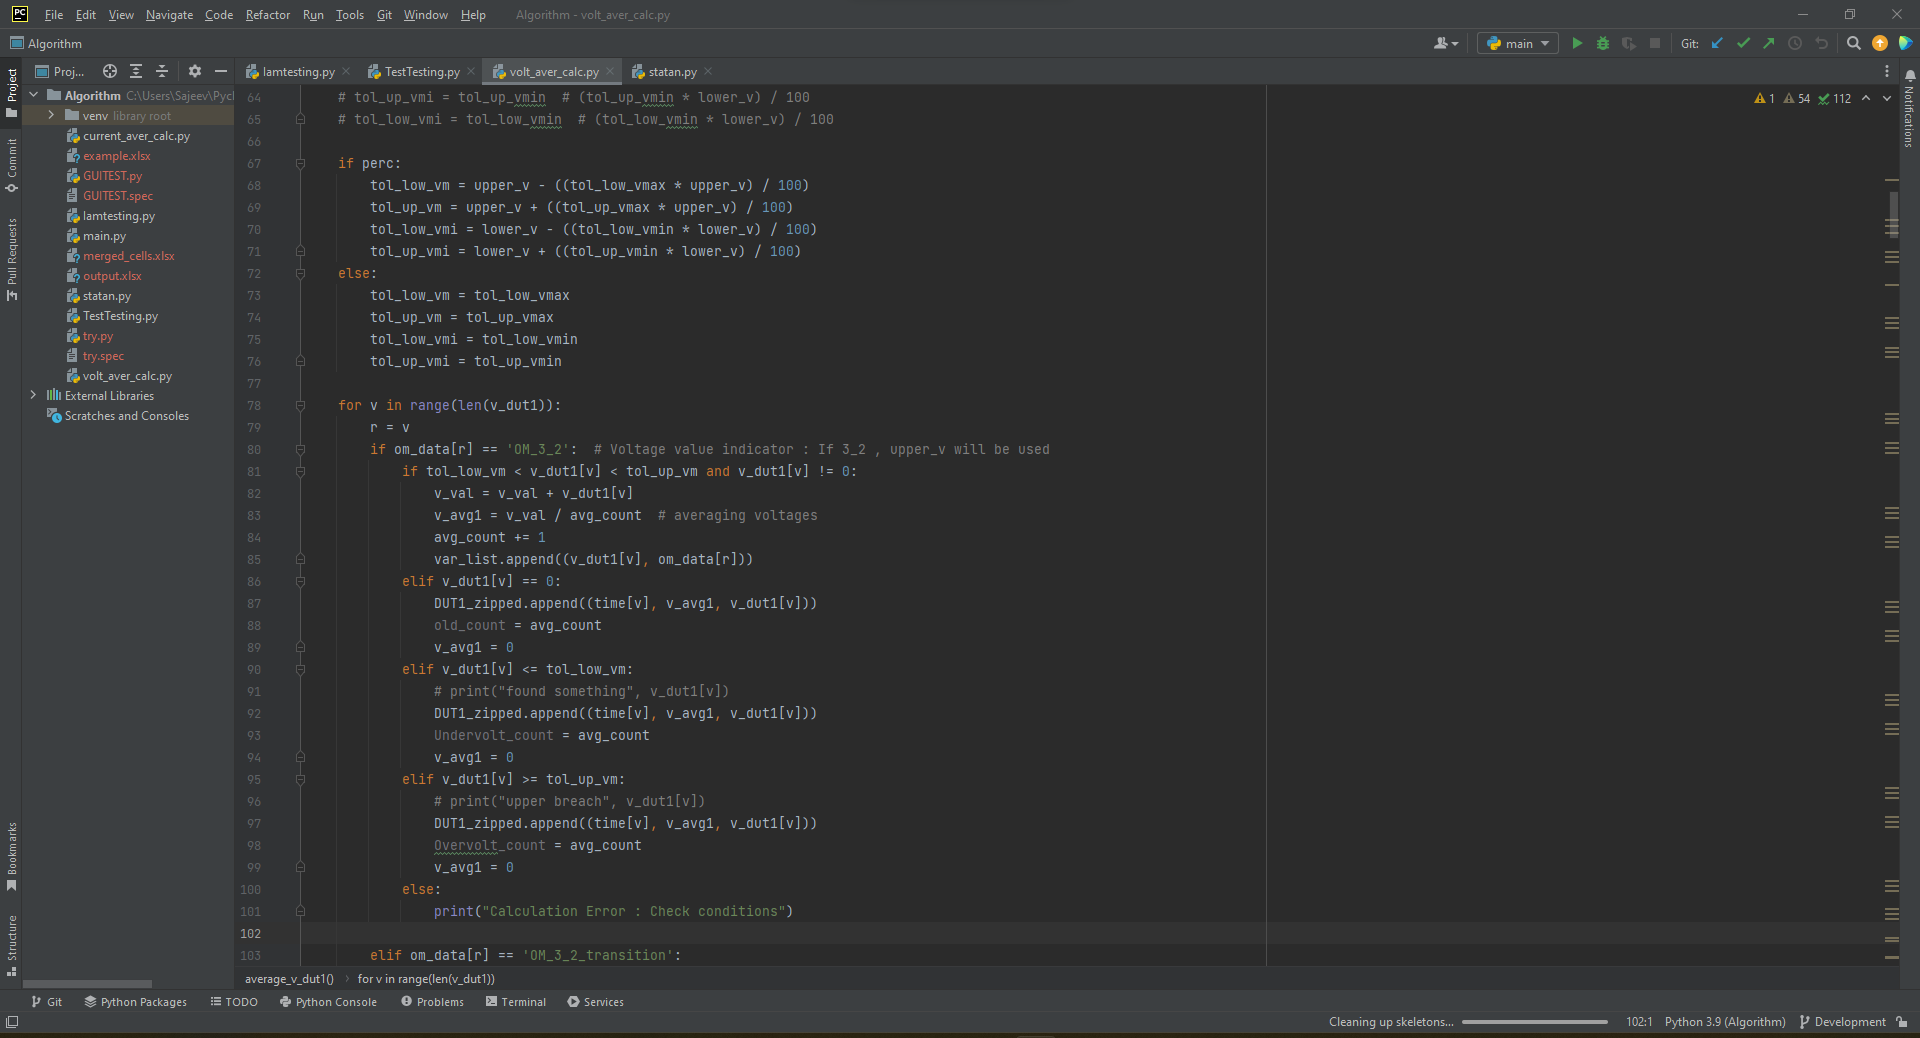
\includegraphics[width= 1\textwidth]{images/pycharm.png}
    \caption [PyCharm]{PyCharm Interface}  
    \label{fig:Pycharm interface}
\end{figure}


The next step in the setup process is to create a project. Whatever you do in PyCharm, you do that in the context of a project. A project is an organizational unit that represents a complete software solution. It serves as a basis for coding assistance, bulk refactoring, coding style consistency, and so on \cite{PyCharm}. The diagram \ref{fig:Project Setup} below shows how to setup the project in PyCharm: 


\begin{figure}[h]
    \centering
    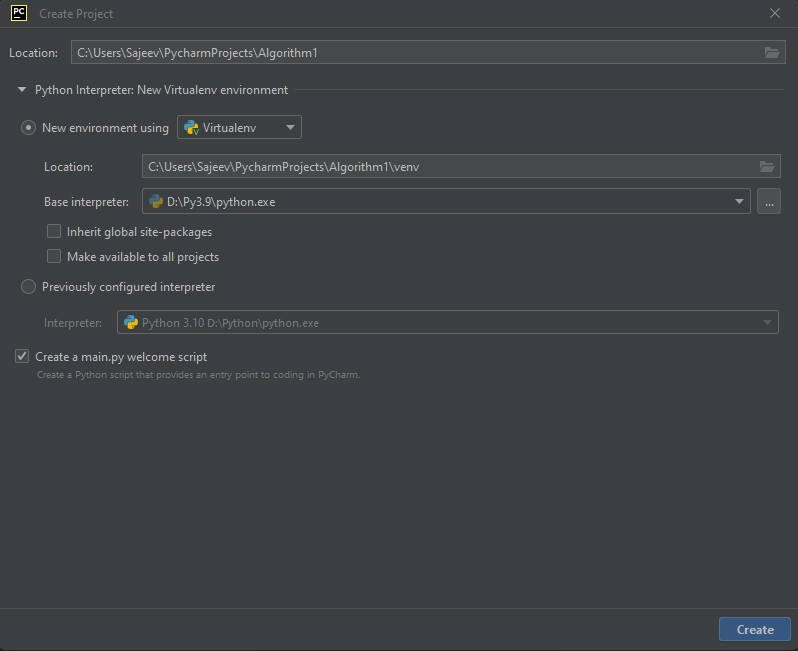
\includegraphics[width= \textwidth]{images/SetupProject.png}
    \caption [Project Setup]{Project Setup}  
    \label{fig:Project Setup}
\end{figure}



The File menu seen in \ref{fig:Pycharm interface} has the option to create new projects, new files, save options as well as load old projects and old files.

PyCharm makes it possible to use the virtualenv tool to create a project-specific isolated virtual environment. The main purpose of virtual environments is to manage settings and dependencies of a particular project regardless of other Python projects. virtualenv tool comes bundled with PyCharm, so the user doesn't need to install it. Rest of the default settings of the setup wizard are accepted as is and a project is created. 

The project creates a main.py file by default which will be the main module of the algorithm. The two sub modules will be defined later in this chapter and will be included in main module via function calls and "import" statements.

\clearpage

\subsection{Primary module}

The main module as shown in the flowchart previously perform the task of data parsing. Data parsing is a method used for giving structure or making sense of unstructured data usually huge files. Usually a part of web development, data parsing is also a part of every industry that deals with huge data-sets and data analysis. Depending on the type of data, various methods are used to separate, filter and structure the data. Here, in this algorithm the user is first asked to specify the source of the test files , which also acts as the destination where the files are stored. Once the source is specified, the user is asked to enter monitoring parameters for the test such a voltage, current values and thereafter also the test duration. The program would be always active for this particular duration. As seen in \ref{fig:Pycharm interface}, the project can be executed with the help of "Run" button. 


The first definitions in every module have to be, implicitly, library or module import definitions. Without these definitions the program won't be able to utilise necessary packages and functions and thus always causing error. 

\begin{lstlisting}[label={lst:import},language=Python]
import os
import itertools
import time
from natsort import natsorted
import voltage_aver_calc
import current_aver_calc
import numpy as np
import pandas as pd
import PySimpleGUI as sg
import statan
import traceback
import sys
import warnings
\end{lstlisting}

Thereafter, comes the definitions for GUI or Graphical User Interface. The GUI pops up as soon as the project is executed. The user input wizard is split in two parts : 

The first window requires the user to input to define the source of the data files to be compressed. Thereafter, the user has the option to define various values like: \[V_{max}, V_{min}, I_{min}, I_{max}\] The user has to also input the duration of test which defines the period of monitoring for the program. Here is the snippet for definition of the GUI : 

\begin{lstlisting}[language=Python]
layout_init = [[sg.Text('Folder path')], [sg.InputText()],
               [sg.Text('Maximum Nominal Voltage in Test (V)')], [sg.InputText()],
               [sg.Text('Minimum Nominal Voltage in Test (V)')], [sg.InputText()],
               [sg.Text('Maximum Nominal Current in Test (A)')], [sg.InputText()],
               [sg.Text('Minimum Nominal Current in Test (A)')], [sg.InputText()],
               [sg.Text('Total Test Run Time (in hrs) ')], [sg.InputText()],
               [sg.Text('How would you like to enter Tolerance Values?')],
               [sg.Button('Percentage')], [sg.Button('Absolute Values')]]
window = sg.Window('Data Compression Program', layout_init)
event_init, values_init = window.read()
window.close()
if event_init == 'Percentage':           # check if user wants percentage input or not
    layout = [
        [sg.Text('Upper Tolerance for Max. Voltage (%)')], [sg.InputText()],
        [sg.Text('Lower Tolerance for Max. Voltage (%)')], [sg.InputText()],
        [sg.Text('Upper Tolerance for Min. Voltage (%)')], [sg.InputText()],
        [sg.Text('Lower Tolerance for Min. Voltage (%)')], [sg.InputText()],
        [sg.Text('Upper Tolerance for Max. Current (%)')], [sg.InputText()],
        [sg.Text('Lower Tolerance for Max. Current (%)')], [sg.InputText()],
        [sg.Text('Upper Tolerance for Min. Current (%)')], [sg.InputText()],
        [sg.Text('Lower Tolerance for Min. Current (%)')], [sg.InputText()],
        [sg.Text('Total DUTs active ')], [sg.InputText()],
        [sg.Submit(), sg.Cancel()]]
    window = sg.Window('Data Compression Program with %', layout, resizable=True)
    event, values = window.read()
    perc = True
elif event_init == 'Absolute Values':      # check if user wants absolute input or not
    layout = [[sg.Text('Upper Tolerance for Max. Voltage (V)')], [sg.InputText()],
              [sg.Text('Lower Tolerance for Max. Voltage (V)')], [sg.InputText()],
              [sg.Text('Upper Tolerance for Min. Voltage (V)')], [sg.InputText()],
              [sg.Text('Lower Tolerance for Min. Voltage (V)')], [sg.InputText()],
              [sg.Text('Upper Tolerance for Max. Current (A)')], [sg.InputText()],
              [sg.Text('Lower Tolerance for Max. Current (A)')], [sg.InputText()],
              [sg.Text('Upper Tolerance for Min. Current (A)')], [sg.InputText()],
              [sg.Text('Lower Tolerance for Min. Current (A)')], [sg.InputText()],
              [sg.Text('Total DUTs active ')], [sg.InputText()],
              [sg.Submit(), sg.Cancel()]]
    window = sg.Window('Data Compression Program with Absolute Values', layout, resizable=True)
    event, values = window.read()
    perc = False
window.close()
\end{lstlisting}

The GUI at execution phase appears as shown below : 

\begin{figure}[h]
    	\centering
    	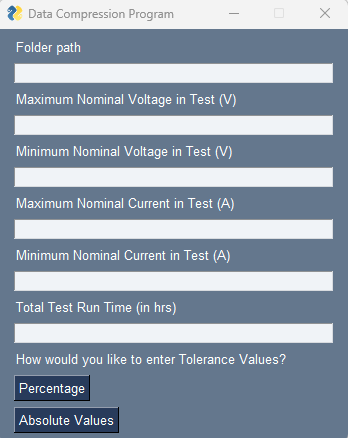
\includegraphics[width= 0.75\textwidth]{images/GUI-1.png}
    	\caption [GUI-I]{User Input}  
    	\label{fig:GUI1}
\end{figure}

Once the user inputs all the values, the user has two options to select the tolerance values, discussed in \ref{sec:Mathematical reduction}, in percentage mode or as absolute values. The user can define asymmetric tolerances with the help of this GUI. While dealing with real-time DUTs it is possible that asymmetric deviation behaviour is observed in real values compared to expected values . Thus, it is reasonable to have the option of defining tolerances in an asymmetric fashion to used later on in the mathematical reduction process.

The following figures represent the user input as percentage mode or as absolute values :

\begin{figure}[!h]
    	\centering
    	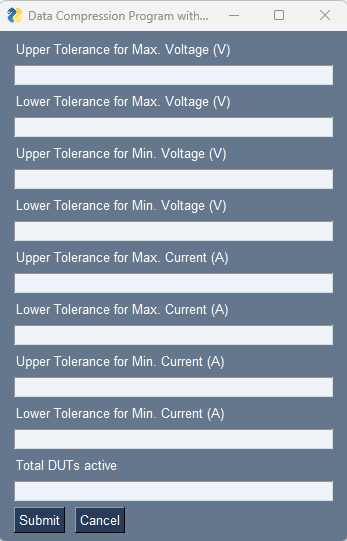
\includegraphics[width= 0.75\textwidth]{images/GUI-Absol.png}
    	\caption [Absolute Values]{Absolute Mode}  
    	\label{fig:Absolute Mode}
\end{figure}

\begin{figure}[!h]
    	\centering
    	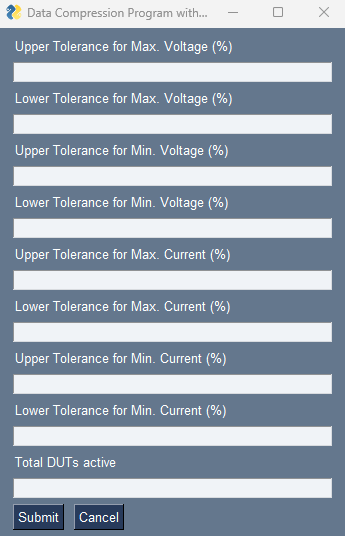
\includegraphics[width= 0.75\textwidth]{images/GUI-perc.png}
    	\caption [Percentage Values]{Percentage Mode}  
    	\label{fig:Percentage Mode}
\end{figure}

\clearpage

Once the user clicks on "Submit" button, the program enters the next phase which is monitoring the target files and folder and data parsing. The program checks every 10 seconds whether a new file is added or not. If no file is added the program enters sleep mode, otherwise it performs data parsing and later on data compression. The user can change this sleep interval, in the source code directly, depending on duration of the test. For example, if the tests are 100s of hours long and the test system generates log files every 6 hours, it doesn't make sense to have a sleep timer of just 10 seconds. Increasing the sleep timer interval will just help saving computing resources of the system where the program gets executed. 

The files are fetched sequentially to be read by the program and parsed. This means that even if multiple files are added in quick succession in the source folder, the program reads them sequentially sorted by name and processes them. The program additionally performs two checks , the first one is whether the file that is being processed has not been processed or handled by the program earlier and second is if it is of '.asc' file format or not. Since the mathematical reduction is designed to be performed on ASCII files, it is essential to keep a check that only ".asc" files are read, parsed and processed. The below code describes the file processing and parsing process:


\begin{lstlisting}[language = Python]
    files = os.listdir(directory)  # file i/o initialisation
    files = natsorted(files)
    for file in files:
        base, ext = os.path.splitext(file)
        if file not in processed_files and ext == '.asc':
            print("File added:", file)
            file_path = os.path.join(directory, file)
            count = 0
            with open(file_path, 'r') as file_in:
                processed_files.append(file)
\end{lstlisting}

Once the individual file is sequentially read and opened by the program, the next step is to parse the data. The parsing of data is also a very complex process because of an undesired mix of datas in the files. The files are typically in the following format : 

\begin{sidewaysfigure}
    	\centering
    	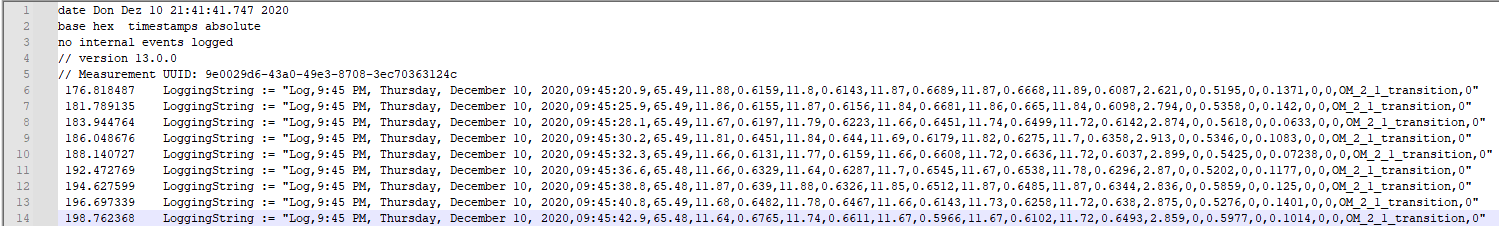
\includegraphics[width=1\textwidth]{images/asc.png}
    	\caption [ASCII data]{Data format}  
    	\label{fig:ascii data}
\end{sidewaysfigure}
\clearpage

As seen in the figure above, the lines 1 to 5 are textual information which are irrelevant for the compressed file. The compressed file must contain information about the parametric behaviour of the DUTs, i.e the voltage \& current characteristics. Thus, these lines can be eliminated via parsing. The main information about test results start from line 6. As seen in the figure, the first column is the value of the logging timer. It shows that the data is logged at an average of about every 2 seconds. This is also irrelevant for the final parsed data since there are timestamps which are part of logging string that indicate the same information. Thus the first column can be eliminated. The column "LoggingString :=" can also be eliminated as it is just a text identifier for the following string. The values from "Log, 9:45 PM," until "OM\_2\_1\_transition" are essential for mathematical reduction as well data evaluation later on. Thus these values will be parsed and saved for use later on in the program. It is visible that the data is split via separators. Similar to ".csv" file, these log file datas are also split by "," separators. Sometimes, there are exceptions and " " (space) is also used as separators. Thus, these separators can be used as flags to split the data into individual columns and then storing as set of data into lists. Lists store multiple items in a single variable. Lists are one of 4 built-in data types in Python used to store collections of data. Python has a very efficient library called pandas which has various functions that deals with data files such as ".csv", ".asc" , ".xlsx" and so on flawlessly. The .read\_csv() \cite{Pandas} function from this library will be used for this split and store process as shown below : \\

\begin{lstlisting}[language = Python]
  # Checks file formatting similar to Excel Text Import Wizard:
  for i, line in enumerate(file_in):
      if "LoggingString" in line:
         val = i
         break 
   print(val)
   df = (pd.read_csv(file_path, sep=',|(?<=[\w"])\s+(?=[\w"])',
                     header=None, skiprows=val, engine="python", on_bad_lines="skip").iloc[:, 2:28])
   df.insert(0, "filename", file.split("\\", )[-1])
   # li.append(df)y
   Output_list = (df.values.tolist())
   for v in range(len(Output_list)):
       Final.append(Output_list[v][7:28])
   for f in Final:  # To convert each element of specific list to float
       for a in range(len(f)):  # Try to include OM column in the data !!!
           if a == 0:
               f[a] = f[a]
           elif 0 < a < 19:
               f[a] = float(f[a])
           elif a == 19:
               f[a] = f[a]
       Data.append(f)
\end{lstlisting}

\subsection{Mathematical Reduction}

Once the data is parsed, it is stored in lists to be passed on to two different functions : 

1) Arithmetic mean of Voltage components  2) Arithmetic mean of Current components

As seen in code snippet \ref{lst:import}, \textbf{voltage\_aver\_calc} and \textbf{current\_aver\_calc} modules are imported into the main module. These are two individual modules that deal with the mathematical reduction. The program design is already clear with the flowchart \ref{fig:Mathematical Reduction}. The parsed data is passed into each of these modules via the functions calls :

\begin{lstlisting}[language = Python]
End_Result_V = voltage_aver_calc.average_v(Data, v_max, v_min, tol_up_vmax, tol_low_vmax, tol_up_vmin, tol_low_vmin, DUT_in, perc)

End_Result_I = current_aver_calc.average_i(Data, i_max, i_min, tol_up_imax, tol_low_imax, tol_up_imin, tol_low_imin, DUT_in, perc)
\end{lstlisting}

\textbf{voltage\_aver\_calc} is a module that is made up of 9 function definitions. The primary function call is \textbf{average\_v} which acts a bridge between the parsed data from main module and the \textbf{average\_v\_dutx} function calls. The "x" in dutx is purely representational and has been replaced by numbers 1 to 8 in the source code to define 8 functions for corresponding DUTs involved in the testing process. 

The \textbf{average\_v} receives various values such as maximum and minimum values of all the voltage levels involved in the testing, total no. of active DUTs in the tests, the tolerances and indicator flag for percentage or absolute values of tolerance. Thereafter, the 8 DUT average functions are evoked from here and the resultant values from each of those functions are concatenated here and returned to the main module. Every function call in python has a return value, which is the output of the function call. The return value of \textbf{average\_v} is a list which contains all the concatenated values. Here is the definition of the \textbf{average\_v} function : \\

\begin{lstlisting}[language = Python]
# Average Function called from main module definition:
 
 
def average_v(Data, v_max, v_min, tol_up_vmax, tol_low_vmax, tol_up_vmin, tol_low_vmin, dut_in, perc):
    V_DUT1, V_DUT2, V_DUT3, V_DUT4, V_DUT5, V_DUT6, V_DUT7, V_DUT8 = ([] for i in range(8))
    Time = []
    Final_List_V = []
    OM_Data = []

#assigning parsed values from file to corresponding parameters:

    for d in Data:    
        Time.append(d[0])
        V_DUT1.append(d[2])
        V_DUT2.append(d[4])
        V_DUT3.append(d[6])
        V_DUT4.append(d[8])
        V_DUT5.append(d[10])
        V_DUT6.append(d[12])
        V_DUT7.append(d[14])
        V_DUT8.append(d[16])
        OM_Data.append(d[19])
 
    functions = [average_v_dut1, average_v_dut2, average_v_dut3, average_v_dut4, 
    average_v_dut5, average_v_dut6, average_v_dut7, average_v_dut8]
 
    for i in range(dut_in):         #invoking averaging function for each DUTs 
        list_name = f"V_DUT{i + 1}"
        V_DUT = locals()[list_name]
        function = functions[i]
        #Concatenate outputs:
        Final_List_V.extend(
            [function(V_DUT, OM_Data, v_max, v_min, tol_up_vmax, tol_low_vmax, tol_up_vmin, tol_low_vmin, Time, perc)])    
    return Final_List_V    
\end{lstlisting}

The next step in this module is calculating arithmetic mean of values for each DUTs. The following code snippet shows the definition of mathematical reduction via arithmetic mean function for DUT1. This is replicated for all the remaining DUTs :
\\
\begin{lstlisting}[language = Python]
def average_v_dut1(v_dut, om_values, upper_v, lower_v, tol_up_vmax,
                    tol_low_vmax ,tol_up_vmin , tol_low_vmin, time, perc):
 
    # Calculating Average of Voltage from DUT 1:
    
    DUT1_avg, DUT1_zipped, DUT1_transitionV = ([] for p in range(3)) #list definition
    var_list = []    #list definition
    time = time
    v_avg1, v_val, v = 0, 0, 0
    avg_count = 1
    v_dut1 = v_dut   #list definition
    om_data = om_values
 
    if perc:       #tolerance definition if percentage mode 
        tol_low_vm = upper_v - ((tol_low_vmax * upper_v) / 100)
        tol_up_vm = upper_v + ((tol_up_vmax * upper_v) / 100)
        tol_low_vmi = lower_v - ((tol_low_vmin * lower_v) / 100)
        tol_up_vmi = lower_v + ((tol_up_vmin * lower_v) / 100)
    else:         #tolerance definition if absolute mode
        tol_low_vm = tol_low_vmax
        tol_up_vm = tol_up_vmax
        tol_low_vmi = tol_low_vmin
        tol_up_vmi = tol_up_vmin
 
    for v in range(len(v_dut1)):
        r = v
        if om_data[r] == 'OM_3_2':  # Voltage value indicator : High performance mode
            if tol_low_vm < v_dut1[v] < tol_up_vm and v_dut1[v] != 0:
                v_val = v_val + v_dut1[v]
                v_avg1 = v_val / avg_count  #averaging voltages
                avg_count += 1
                var_list.append((v_dut1[v], om_data[r]))
            elif v_dut1[v] == 0:
                DUT1_zipped.append((time[v], v_avg1, v_dut1[v]))
                old_count = avg_count
                v_avg1 = 0
            elif v_dut1[v] <= tol_low_vm:
                DUT1_zipped.append((time[v], v_avg1, v_dut1[v]))
                Undervolt_count = avg_count
                v_avg1 = 0
            elif v_dut1[v] >= tol_up_vm:
                DUT1_zipped.append((time[v], v_avg1, v_dut1[v]))
                Overvolt_count = avg_count
                v_avg1 = 0
            else:
                print("Calculation Error : Check conditions")
 
        elif om_data[r] == 'OM_3_2_transition':  #Operation mode change. No averaging here
            DUT1_transitionV.append(v_dut1[v])
 
        elif om_data[r] == 'OM_2_1':  #Voltage value indicator : Normal / Sleep mode
            if tol_low_vmi < v_dut1[v] < tol_up_vmi and v_dut1[v] != 0:
                v_val = v_val + v_dut1[v]
                v_avg1 = v_val / avg_count  #averaging voltages
                avg_count += 1
                var_list.append((v_dut1[v], om_data[r]))
            elif v_dut1[v] == 0:
                DUT1_zipped.append((time[v], v_avg1, v_dut1[v]))
                old_count = avg_count
                v_avg1 = 0
            elif v_dut1[v] <= tol_low_vmi:
                DUT1_zipped.append((time[v], v_avg1, v_dut1[v]))
                undervolt_count = avg_count
                v_avg1 = 0
            elif v_dut1[v] >= tol_up_vmi:
                DUT1_zipped.append((time[v], v_avg1, v_dut1[v]))
                overvolt_count = avg_count
                v_avg1 = 0
            else:
                print("Calculation Error : Check conditions")
 
        elif om_data[r] == 'OM_2_1_transition': #Operation mode change. No averaging here
            DUT1_transitionV.append(v_dut1[v])
 
        else:
            print("Unknown Operation Mode")
 
    DUT1_avg.append(v_avg1)
    return DUT1_avg, DUT1_zipped, DUT1_transitionV, var_list
\end{lstlisting}

The first part of the code snippet above is function definition. The function receives all necessary values such as voltage, operation mode values, V\_max, V\_min, tolerances for both levels, timestamp values and flag for tolerance mode from the \textbf{average\_v} function. Thereafter, depending on the indicator flag for tolerance mode, the tolerances are calculated for each levels of voltage. From line 25 in the snippet, the calculation of arithmetic mean begins. The calculation of arithmetic mean has been so designed that depending on the operation mode, the voltage levels and their corresponding tolerance levels will be activated via conditional checks. If the value of voltages lie between the set tolerance values and not equal to zero, it is included in the arithmetic mean calculation and then the average counter, \textbf{avg\_count} is incremented. 

The purpose for the algorithm is to reduce the size of error free data and evaluate it. Hence, the conditional checks are implemented to filter out the error free values for reducing, also called as clipping. The values that are outside the tolerance zones are not discarded since they are of importance for the test engineer to evaluate the cause and type of errors in the test system. It is important to show the time and magnitude of error for the engineer to make sense out of it. Thus, in the conditional checks where DUT voltages lie outside the tolerance ranges or are equal to 0, a new list is concatenated or appended with the time stamp of occurrence of the error, average value just prior to occurrence of the error and the magnitude of the error. The average value is then set to 0 after every error occurrence, to ensure that the final average/mean of error free values do not contain any garbage values. The averaging function conducts a total 5 conditional checks on the operation mode of the test data. Depending on the operation mode, the calculation process is carried out. 

Once the error free values are filtered and averaged, it is also important to find the variance of the values in order to find the spread of the error free data. Even though, the filtered data lie inside desired range of tolerances the calculation of variance helps to understand how close or far away are the values in general from the average of the voltage and current values. The arithmetic mean is not a good indicator of the spread of the values in a range, however, variance is a good indicator of this phenomenon. Thus a new list \textbf{var\_list} is appended to contain the filtered voltage values and the operation mode value. They are processed in the statistical analysis module of the program, explained later in this thesis. 

Once all the calculations are carried out the \textbf{average\_v\_dut1} function returns 4 lists as result of the calculation process. The first list is a list of final average of the DUT, list of improper values and indicators, list of transition voltage values and finally the list that contain error free value for statistical analysis.

Now that average calculation of the voltage component is explained, below is the code snippet for average calculation of the current component. The code and design is similar to the voltage component average with just minor changes related to the naming or current parameters of the testing system.\\

\begin{lstlisting}[language = Python]
# Average Function called from main module definition :
 
def average_i(Data, i_max, i_min, tol_up_imax, tol_low_imax, tol_up_imin, tol_low_imin, dut_in, perc):
 
    Final_List_I, OM_Data = [], []
    I_DUT1, I_DUT2, I_DUT3, I_DUT4, I_DUT5, I_DUT6, I_DUT7, I_DUT8 = ([] for i in range(8))
    Time = []
    
    #assigning parsed values from file to corresponding parameters:
    
    for d in Data:
        Time.append(d[0])
        I_DUT1.append(d[3])
        I_DUT2.append(d[5])
        I_DUT3.append(d[7])
        I_DUT4.append(d[9])
        I_DUT5.append(d[11])
        I_DUT6.append(d[13])
        I_DUT7.append(d[15])
        I_DUT8.append(d[17])
        OM_Data.append(d[19])
 
    functions = [average_i_dut1, average_i_dut2, average_i_dut3, average_i_dut4, average_i_dut5, average_i_dut6,
                 average_i_dut7, average_i_dut8]
                 
    for i in range(dut_in):   #invoking averaging function for each DUTs
        list_name = f"I_DUT{i + 1}"
        I_DUT = locals()[list_name]
        function = functions[i]
        Final_List_I.extend(
            [function(I_DUT, OM_Data, i_max, i_min, tol_up_imax, tol_low_imax, tol_up_imin, tol_low_imin, Time, perc)])
 
    return Final_List_I

#--------------------------------------------------------------------
#Averaging of current values from different DUTs:
 
def average_i_dut1(i_dut, om_values, upper_a, lower_a, tol_up_imax, 
                    tol_low_imax, tol_up_imin, tol_low_imin, time, perc):
 
    # Calculating Average of Current from DUT 1:
 
    DUT1_avg, DUT1_izipped, DUT1_transitioni = [], [], []
    time = time
    var_list = []
    i_avg1, i_val, i = 0, 0, 0
    avg_count = 1
    i_dut1 = i_dut
    om_data = om_values
    if perc:
        tol_low_im = upper_a - ((tol_low_imax * upper_a) / 100)
        tol_up_im = upper_a + ((tol_up_imax * upper_a) / 100)
        tol_low_imi = lower_a - ((tol_low_imin * lower_a) / 100)
        tol_up_imi = lower_a + ((tol_up_imin * lower_a) / 100)
    else:
        tol_low_im = tol_low_imax
        tol_up_im = tol_up_imax
        tol_low_imi = tol_low_imin
        tol_up_imi = tol_up_imin
    for i in range(len(i_dut1)):
        r = i
        if om_data[r] == 'OM_3_2':
            if tol_low_im < i_dut1[i] < tol_up_im and i_dut1[i] != 0:
                i_val = i_val + i_dut1[i]
                i_avg1 = i_val / avg_count
                avg_count += 1
                var_list.append((i_dut1[i], om_data[r]))
            elif i_dut1[i] == 0:
                DUT1_izipped.append((time[i], i_avg1, i_dut1[i]))
                old_count_zero = avg_count
                i_avg1 = 0
            elif i_dut1[i] <= tol_low_im:
                DUT1_izipped.append((time[i], i_avg1, i_dut1[i]))
                Undercurrent_count = avg_count
                i_avg1 = 0
            elif i_dut1[i] >= tol_up_im:
                DUT1_izipped.append((time[i], i_avg1, i_dut1[i]))
                Overcurrent_count = avg_count
                i_avg1 = 0
            else:
                print("Calculation Error : Check conditions")
 
        elif om_data[r] == 'OM_3_2_transition':
            DUT1_transitioni.append(i_dut1[i])
 
        elif om_data[r] == 'OM_2_1':
            if tol_low_imi < i_dut1[i] < tol_up_imi and i_dut1[i] != 0:
                i_val = i_val + i_dut1[i]
                i_avg1 = i_val / avg_count
                avg_count += 1
                var_list.append((i_dut1[i], om_data[r]))
            elif i_dut1[i] == 0:
                DUT1_izipped.append((time[i], i_avg1, i_dut1[i]))
                old_count = avg_count
                i_avg1 = 0
            elif i_dut1[i] <= tol_low_imi:
                DUT1_izipped.append((time[i], i_avg1, i_dut1[i]))
                Undercurrent_count = avg_count
                i_avg1 = 0
            elif i_dut1[i] >= tol_up_imi:
                DUT1_izipped.append((time[i], i_avg1, i_dut1[i]))
                Overcurrent_count = avg_count
                i_avg1 = 0
            else:
                print("Calculation Error : Check conditions")
 
        elif om_data[r] == 'OM_2_1_transition':
            DUT1_transitioni.append(i_dut1[i])
 
        else:
            print("Unknown Operation Mode")
    DUT1_avg.append(i_avg1)
    return DUT1_avg, DUT1_izipped, DUT1_transitioni, var_list
\end{lstlisting}

\subsection{Statistical Analysis}\label{sec:StatAn}

Once the mathematical reduction is performed, the main module receives values from the voltage and current components. From these results, some parts are passed on to another module known as \textbf{statan.py}. This module deals with data evaluation of the reduced data for the engineer to have better understanding of the error free data-sets. Two types of data evaluation is conducted with this module : 

1) Variance or Spread of Data \\ 2) Drift Representation

\paragraph{Variance:}

Variance is a measure of dispersion, meaning it is a measure of how far a set of numbers is spread out from their average value \cite{Var}. It is an important measure to show how far the error free values are spread from the mean value in the tolerance window defined by the user. The variance is the the sum of squared deviations from the mean. It is denoted by : 

\begin{equation}
s^2 = \frac{1}{n-1} \sum_{i=1}^{n} (x_i - \bar{x})^2
\end{equation}

The code snippet below shows how the variance is calculate from the main module via a function call to the statan.py module : \\

\begin{lstlisting}[language = Python]
import numpy as np
import statistics


var_v1, var_v2, var_i1, var_i2, = [], [], [], []
for d in range(DUT_in):
     v1, v2 = statan.var(End_Result_V[d][3])  #pass the list of error free voltage values to the function
     i1, i2 = statan.var_current(End_Result_I[d][3]) #pass the list of error free current values to the function
     var_v1.append(v1)
     var_v2.append(v2)
     var_i1.append(i1)
     var_i2.append(i2)
\end{lstlisting}


The above function call invokes the statan.py module and the variance function for voltage and current and calculates 
variance and returns the values . It is represented in the code snippet below : 

\begin{lstlisting}[language = Python]

#Variance of Voltage components :
def var(var_list):
    var_2_1 = []  #list for sleep mode values
    var_3_2 = []  #list for performance mode values 
    var2, var3 = 0, 0
    for i, element in enumerate(var_list):
        val, om_data = element
        if om_data == 'OM_2_1':  #list appended if DUT in sleep mode
            var_2_1.append(val)     
        elif om_data == 'OM_3_2': #list appended if DUT in performance mode
            var_3_2.append(val)
    if len(var_2_1) > 1:     #check to ensure atleast 2 values are present in list to calculate variance
        var2 = statistics.variance(var_2_1)
    if len(var_3_2) > 1:      #check to ensure atleast 2 values are present in list to calculate variance
        var3 = statistics.variance(var_3_2)
    return var2, var3       #return variance values
 
 #Variance of Current components :
def var_current(var_list):
    var_2_1 = []     #list for sleep mode values
    var_3_2 = []     #list for performance mode values
    var2, var3 = 0, 0
    for i, element in enumerate(var_list):
        val, om_data = element
        if om_data == 'OM_2_1': #list appended if DUT in sleep mode
            var_2_1.append(val)
        elif om_data == 'OM_3_2': #list appended if DUT in performance mode
            var_3_2.append(val)
    if len(var_2_1) > 1:  #check to ensure atleast 2 values are present in list to calculate variance
        var2 = statistics.variance(var_2_1)
    if len(var_3_2) > 1:  #check to ensure atleast 2 values are present in list to calculate variance
        var3 = statistics.variance(var_3_2)
    return var2, var3       #return variance values
\end{lstlisting}


\paragraph{Drift representation:} Drift analysis is an important tool to understand the lifetime behaviour of a component. Devices of any type, shape or purpose endure wear and tear with prolonged usage and thus their functionalities is affected. If the devices work under tolerance limits, it is essential to understand the drift behaviour so that timely calibration can be conducted thus preventing malfunctioning of the device or damage caused by the device. 

Every device is designed to work along specified or desired value of a parameter along with the tolerance limits. For e.g, Multi-meters. These devices are designed and calibrated to measure various parameters such as voltage, current, resistance, temperature etc. with great precision. However, due to it being an electronic device the internal components are going to experience degradation over time. This means that the operating values of different parameters would have shifted above or below the desired operating values. If it is within the tolerance windows set for those parameters, there will be no troubles as the measured values will be slightly deviated from original but still within the tolerance range. However, if the deviation is strong then the device will malfunction and thus cause possible damages to the user or provided improper measurements. If the technician is notified of the drift phenomenon in a multi-meter, the device can be calibrated or replaced before it creates any significant problem to it's users.

The drift is usually calculated by selecting a desired value, which is set a reference value and measuring the output values/measured values against the reference. If the measure values = desired value, it can be said that there is not drifting. However, if the measured values fall below or rise above desired range it can be said device has a drift and needs monitoring. The other method to measure a drift is to observe it graphically. The graphical representation of a parameter along the representations is the simplest method to showcase whether a system is experiencing a drift or not.

In this module, the drift is calculated by finding the mean of samples of values and then later on plotting these mean values with respect to the reference value. The option to divide the the data-set into samples before calculating mean or drift is because the data-set is usually very huge. If in the ideal case of zero error occurring during the test phase, the data-set here would consist all the values of the log file which would make it extremely huge to deal with. Hence, a sample size is selected to quantize chunks of data into single values and then plot them to observe the drift in the system. 

Below is the snippet for the code calculating the mean of the samples : 

\begin{lstlisting}[language = Python]
# Drift Analysis of the Voltage values:

count = 50
 
def drift_an(data, v_max, v_min): 
    std_2_1, std_3_2 = [], []
    dat_2_1 = []
    dat_3_2 = []
    remaining = []
    for i, element in enumerate(data):
        val, om_data = element
        if om_data == 'OM_2_1': #list appended if DUT in sleep mode
            dat_2_1.append(val)
        elif om_data == 'OM_3_2': #list appended if DUT in performance mode
            dat_3_2.append(val)
    if len(dat_2_1) > 0:          #list should contain atleast 1 element
        group_num = len(dat_2_1) // count    #Total samples of size "count"
        remaining_group = len(dat_2_1) % count  #Remaining sample group size
        for i in range(0, group_num * count, count):
            group = dat_2_1[i:i + count]
            std_2_1.append(np.mean(group))      #calculate mean of each group
        if remaining_group != 0:
            for j in range((len(dat_2_1) - remaining_group), len(dat_2_1)):
                remaining.append(dat_2_1[j])
            std_2_1.append(np.mean(remaining)) #calculate mean of remaining group
        else:
            print("Check Finished")
    if len(dat_3_2) > 0:
        group_num = len(dat_3_2) // count
        remaining_group = len(dat_3_2) % count
        for i in range(0, group_num * count, count):
            group = dat_3_2[i:i + count]
            std_3_2.append(np.mean(group))
        if remaining_group != 0:
            for j in range((len(dat_3_2) - remaining_group), len(dat_3_2)):
                remaining.append(dat_3_2[j])
            std_3_2.append(np.mean(remaining))
        else:
            print("Check Finished")
    return std_2_1, std_3_2
 
# Drift Analysis of the Current values:
 
def drift_an_current(data, i_max, i_min):
    std_2_1, std_3_2 = [], []
    dat_2_1 = []
    dat_3_2 = []
    remaining = []
    for i, element in enumerate(data):
        val, om_data = element
        if om_data == 'OM_2_1':
            dat_2_1.append(val)
        elif om_data == 'OM_3_2':
            dat_3_2.append(val)
    if len(dat_2_1) > 0:
        group_num = len(dat_2_1) // count       #Total samples of size "count"
        remaining_group = len(dat_2_1) % count  #Remaining sample group size
        print("len", len(dat_2_1), "remg", remaining_group)
        for i in range(0, group_num * count, count):
            group = dat_2_1[i:i + count]
            std_2_1.append(np.mean(group))    #calculate mean of each group
        if remaining_group != 0:
            for j in range((len(dat_2_1) - remaining_group), len(dat_2_1)):
                remaining.append(dat_2_1[j])
            std_2_1.append(np.mean(remaining))  #calculate mean of remaining group
        else:
            print("Check finished")
    if len(dat_3_2) > 0:
        group_num = len(dat_3_2) // count
        remaining_group = len(dat_3_2) % count
        print("len", len(dat_3_2), "remg", remaining_group)
        for i in range(0, group_num * count, count):
            group = dat_3_2[i:i + count]
            std_3_2.append(np.mean(group))
        if remaining_group != 0:
            for j in range((len(dat_3_2) - remaining_group), len(dat_3_2)):
                remaining.append(dat_3_2[j])
            std_3_2.append(np.mean(remaining))
        else:
            print("Check finished")
    return std_2_1, std_3_2
\end{lstlisting}

\clearpage
Both these functions return lists of mean values to their respective function calls in the main module. This is shown here : 

\begin{lstlisting}[language = Python]
for dut in range(DUT_in):
   if dut == 0:
      drift1_21, drift1_32 = statan.drift_an(End_Result_V[dut][3], v_max, v_min)
      drifti1_21, drifti1_32 = statan.drift_an_current(End_Result_I[dut][3], i_max, i_min)
   if dut == 1:
      drift2_21, drift2_32 = statan.drift_an(End_Result_V[dut][3], v_max, v_min)
      drifti2_21, drifti2_32 = statan.drift_an_current(End_Result_I[dut][3], i_max, i_min)
   if dut == 2:
      drift3_21, drift3_32 = statan.drift_an(End_Result_V[dut][3], v_max, v_min)
      drifti3_21, drifti3_32 = statan.drift_an_current(End_Result_I[dut][3], i_max, i_min)
   if dut == 3:
      drift4_21, drift4_32 = statan.drift_an(End_Result_V[dut][3], v_max, v_min)
      drifti4_21, drifti4_32 = statan.drift_an_current(End_Result_I[dut][3], i_max, i_min)
   if dut == 4:
      drift5_21, drift5_32 = statan.drift_an(End_Result_V[dut][3], v_max, v_min)
      drifti5_21, drifti5_32 = statan.drift_an_current(End_Result_I[dut][3], i_max, i_min)
   if dut == 5:
      drift6_21, drift6_32 = statan.drift_an(End_Result_V[dut][3], v_max, v_min)
      drifti6_21, drifti6_32 = statan.drift_an_current(End_Result_I[dut][3], i_max, i_min)
   if dut == 6:
      drift7_21, drift7_32 = statan.drift_an(End_Result_V[dut][3], v_max, v_min)
      drifti7_21, drifti7_32 = statan.drift_an_current(End_Result_I[dut][3], i_max, i_min)
   if dut == 7:
      drift8_21, drift8_32 = statan.drift_an(End_Result_V[dut][3], v_max, v_min)
      drifti8_21, drifti8_32 = statan.drift_an_current(End_Result_I[dut][3], i_max, i_min)
\end{lstlisting}

With this all the necessary calculations, compression and processing of data from each file is completed. The next step is to output these results so that the user/engineer could analyse and evaluate the outcome of the complete program:


As mentioned previously at multiple occasions, python is a very efficient language not just in handling and arithmetically processing huge data-sets but also in read, write and storing as different file types. Ms Excel is the most commonly used tool for the purpose of analysing, observing and evaluating numerical data such as the log files handled by python here. Since python has many packages that enable writing data into Excel files, this option was selected to write and store all the processed data from above. 

For every ".asc" filed read by the program, one corresponding ".xlsx" workbook is written back into the source folder. Each workbook consists of three worksheets consisting of:\\
1) Arithmetically reduced data-set\\
2) Variance of the data-set \\
3) Drift Representation of the data-set

The below figures show worksheets from one such compressed data-log workbook :

\begin{sidewaysfigure}
    	\centering
    	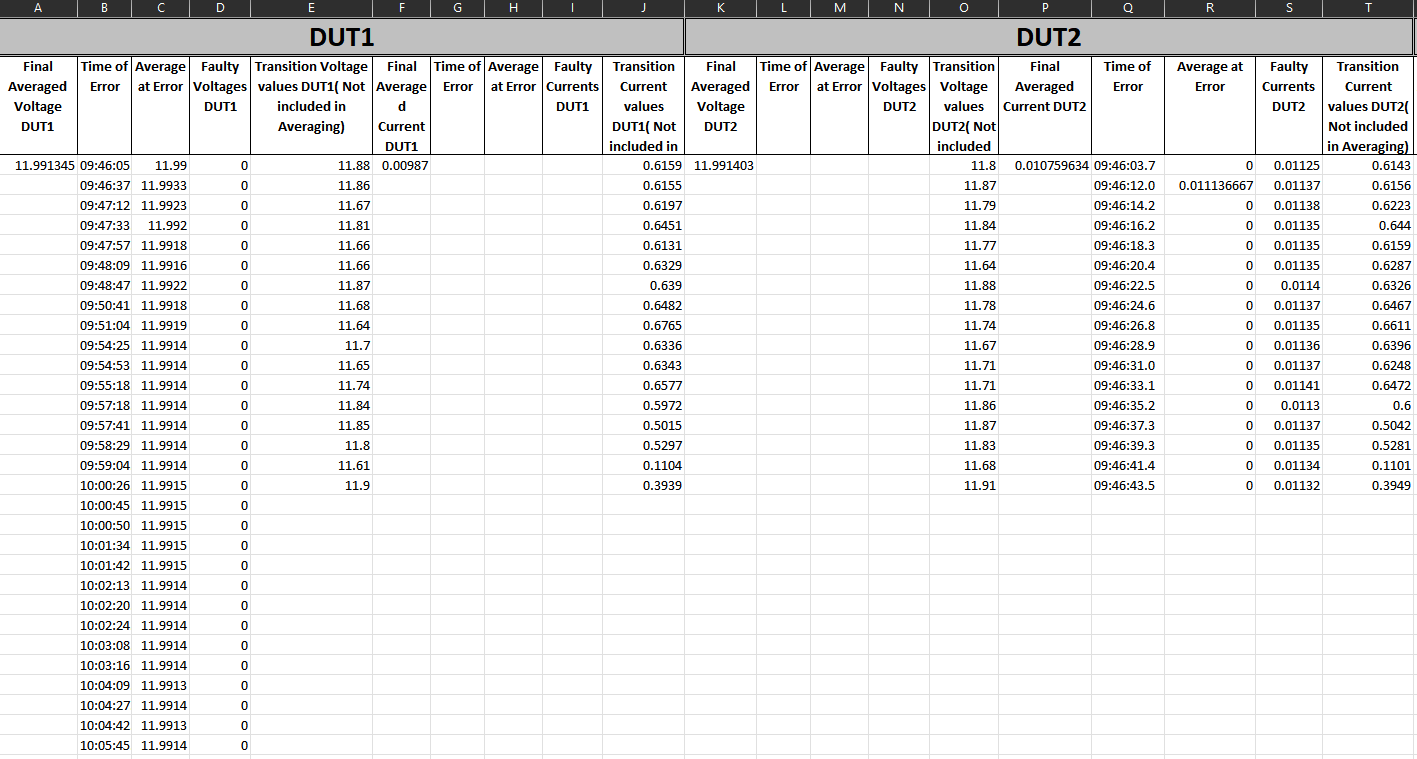
\includegraphics[width= 1\textwidth]{images/Worksheet 1.png}
    	\caption [Reduced Data]{Reduced Data}  
    	\label{fig:Reduced Data}
\end{sidewaysfigure}

The above figure shows an excerpt from the worksheet that shows the compressed version of the log files. As seen in the image, the compressed version is divided in sections based on the DUTs in the log files. Here is the image the data from DUT 1 and DUT 2 is shown. The first column of each section is the final averaged value of the error free values, i.e voltage . The second column is for the Time stamps which indicate at which point of the test run, an error occurred. The column thereafter shows the average value of the system when an error was detected followed by the error value. The final column shows the transition voltages. The transition voltages occur when the DUT switches from one operation mode to the other. They are represented as is and are not part of the average calculation. The same categorisation applies to current values as well. 

The benefit of the algorithm could be seen in the values of DUT 1 and DUT 2. DUT 1 has relatively way more errors than DUT 2. DUT 2 had an almost ideal behaviour during the test run and thus achieved the most level of compression as compared to DUT 1 values. 

\begin{figure}[htbp]
    	\centering
    	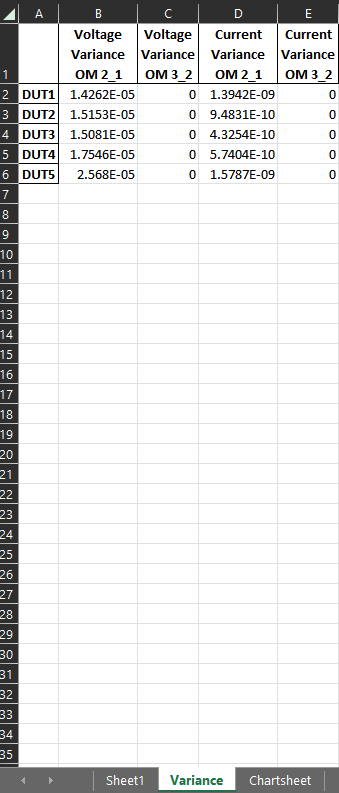
\includegraphics[width= 0.6\textwidth]{images/Variance.png}
    	\caption [Variance]{Variance}  
    	\label{fig:Variance}
\end{figure}

The figure \ref{fig:Variance} below shows the values of variance of the different parameters of the DUTs used in the test. The low value of variance indicates that the data-points are not spread far away from the mean of error free data-set. The lower the value of variance the more stable it could be said the behaviour of the DUT is. 

The images \ref{fig:Drift I} and \ref{fig:Drift II} correspond to the voltage values and current values respectively. Here, the graphical representation of the mean of the samples mentioned in \ref{sec:StatAn} is shown. Each images have corresponding reference value lines against which rest of the lines are plotted. From the \ref{fig:Drift I} it can be seen that each DUT has oscillations but they are not very significant as they lie below the reference value of 12 V . Also, they are the error free values derived from reduction process, which mean they are never out of tolerance windows. All DUTs except for DUT 5 show uniform behaviour. DUT 5 has multiple abnormal oscillations. Even though all of these occur in the tolerance windows, such representations helps the engineer understand the behaviour of the devices in a much more real sense. 

Similarly for the current drift chart, except for DUT 1 and 5, all other DUTs are away from the reference value of 0.01 A. The DUTs 3 and 4 have almost similar behaviour, with DUT 2 having slight oscillations at some points. The DUT 1 and 5 have a totally different behaviours, they have extremely high deflection in the beginning of the test , however they subside over time and become much more stable and closer to the reference line. 

The drift representation is thus helpful in analysing the behaviour of different DUTs over time. 
\begin{figure}[h]
    	\centering
    	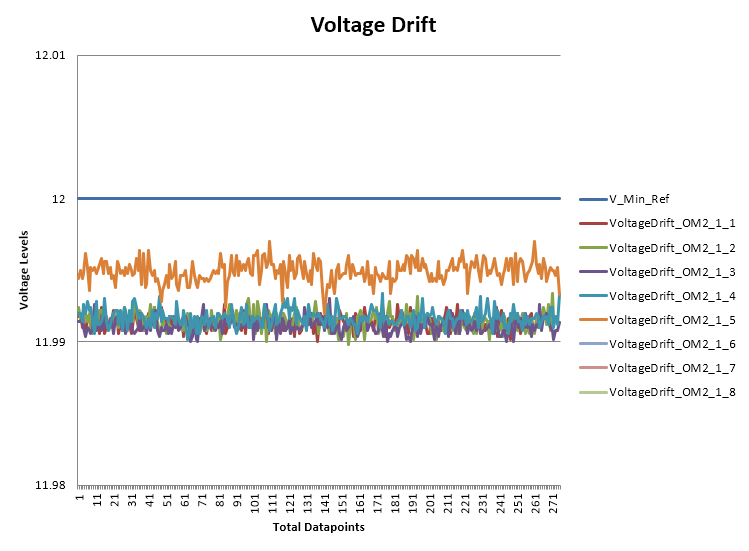
\includegraphics[width= 0.8\textwidth]{images/Voltagedrift.png}
    	\caption [Voltage Drift]{Voltage Drift}  
    	\label{fig:Drift I}
\end{figure}

 

\begin{figure}[h]
    	\centering
    	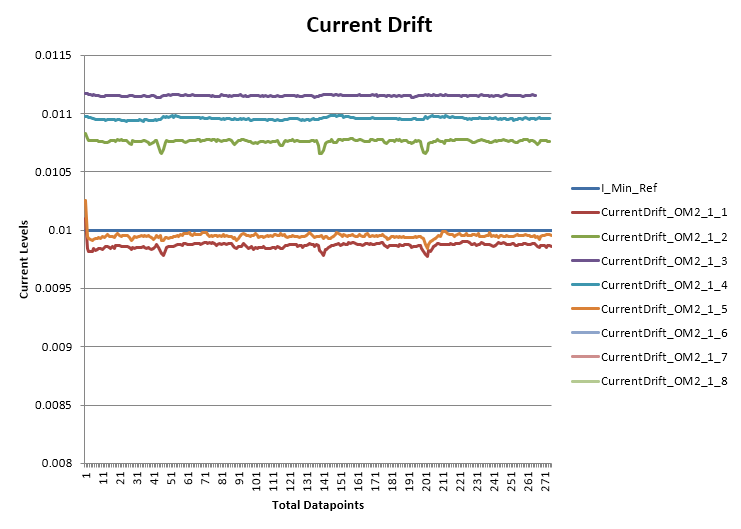
\includegraphics[width= 0.8\textwidth]{images/Currentdrift.png}
    	\caption [Current Drift]{Current Drift}  
    	\label{fig:Drift II}
\end{figure}
\clearpage

\begin{figure}[h]
    	\centering
    	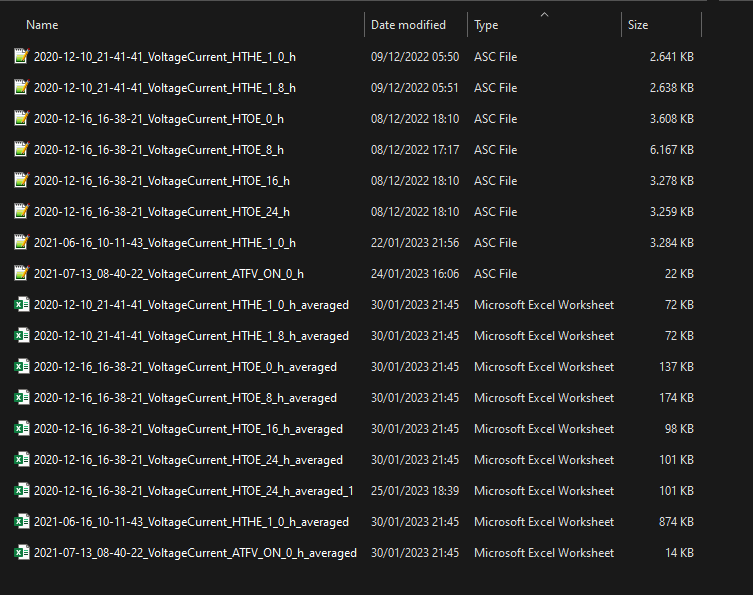
\includegraphics[width= 0.8\textwidth]{images/Size Comparison.png}
    	\caption [Comparison of Size]{Reduced Size}  
    	\label{fig:Size Data}
\end{figure}

The above diagram is a representation of the effectiveness of the compression algorithm. The largest file had a reduction from 6,167 KB to 174 KB. This is a reduction in size by almost 97\%. This would suffice to say that the algorithm is successful in achieving the maximum possible compression. One question might arise as to why are different files of almost similar files sizes have different sizes in their reduced version. As seen in diagram \ref{fig:Reduced Data}, every DUT has different behaviour compared to each other. This means that it is possible in some cases the DUT works perfectly between tolerance limits and thus achieves the most compression, however in some scenarios the DUT works very differently and thus has more errors. This means desired compression cannot be achieved since error values are important indicators of system behaviour and cannot be discarded for the sake of achievement of compression. Thus, many files inspite of having almost similar original file size, have varied file size in reduced form. 

%\input{chap9x} %chap9_futurework_limitations}